\documentclass[ngerman,a4paper,order=firstname]{local_mathscript} %TODO local mathscript to fix counting for STOCH! temp solution.
%{../../texmf/tex/latex/mathscript/mathscript}
\usepackage{../../texmf/tex/latex/mathoperators/mathoperators}

%local packages
\usepackage{cancel}

\title{\textbf{Stochastik SS 2019}}
\author{Dozent: Prof. Dr. \person{Anita Behme}}

% local commands
\renewcommand{\F}{\mathscr F}
\renewcommand{\P}{\mathbb{P}}
\renewcommand{\O}{\Omega}
\renewcommand{\G}{\mathscr{G}}
\newcommand{\Gen}{\mathcal{E}}
\newcommand{\E}{\mathbb{E}}
\newcommand{\Var}{\mathbb{V}\text{ar}}   % Varianz
\newcommand{\Cov}{\mathbb{C}\text{ov}}   % Kovarianz
\newcommand{\Corr}{\mathbb{C}\text{orr}}   % Korrelation
%\newcommand{\Rd}{\R^d}
\def\upmodels{\perp\!\!\!\perp}

\begin{document}
\pagenumbering{roman}
\pagestyle{plain}

\maketitle

\hypertarget{tocpage}{}
\tableofcontents
\bookmark[dest=tocpage,level=1]{Inhaltsverzeichnis}

\pagebreak
\pagenumbering{arabic}
\pagestyle{fancy}

\chapter*{Vorwort}
Schön, dass du unser Skript für die Vorlesung \textit{Lineare Algebra und analytische Geometrie 1} bei Prof. Dr. Arno Fehm im WS2017/18 gefunden hast! \footnote{Obwohl man sagen kann, dass es in dieser Vorlesung nur um Lineare Algebra ging, der Teil mit der analytischen Geometrie wurde vernachlässigt. Liegt wahrscheinlich auch daran, dass es demnächst eine Reform der Studienordnung gibt, in der aus der Vorlesung \textit{Lineare Algebra und analytische Geometrie} die Vorlesung \textit{Einführung in die Lineare Algebra} wird.}

Wir verwalten dieses Skript mittels Github \footnote{Github ist eine Seite, mit der man Quelltext online verwalten kann. Dies ist dahingehend ganz nützlich, dass man die Quelltext-Dateien relativ einfach miteinander synchronisieren kann, wenn man mit mehren Leuten an einem Projekt arbeitet.}, d.h. du findest den gesamten \LaTeX-Quelltext auf \url{https://github.com/henrydatei/TUD_MATH_BA}. Unser Ziel ist, für alle Pflichtveranstaltungen von \textit{Mathematik-Bachelor} ein gut lesbares Skript anzubieten. Für die Programme, die in den Übungen zur Vorlesung \textit{Programmieren für Mathematiker} geschrieben werden sollen, habe ich ein eigenes Repository eingerichtet; es findet sich bei \url{https://github.com/henrydatei/TU_PROG}.

Du kannst dir gerne dort die \LaTeX-Quelldateien herunterladen, die Dateien für exakt dieses Skript sind im Ordner \texttt{1. Semester/LAAG ueberarbeitet}. Es lohnt sich auf jeden Fall während des Studiums die Skriptsprache \LaTeX{} zu lernen, denn Dokumente, die viele mathematische oder physikalische Formeln enthalten, lassen sich sehr gut mittels \LaTeX{} darstellen, in Word oder anderen Office-Programmen sieht so etwas dann eher dürftig aus.

\LaTeX{} zu lernen ist gar nicht so schwierig, ich habe dafür am Anfang des ersten Semesters wenige Wochen benötigt, dann kannte ich die wichtigsten Befehle und konnte den Vorgänger dieses Skriptes schreiben (\texttt{1. Semester/LAAG}, Vorsicht: hässlich, aber der Quelltext ist relativ gut verständlich).

Es sei an dieser Stelle darauf hingewiesen (wie in jedem anderem Skript auch \smiley{}), dass dieses Skript nicht den Besuch der Vorlesungen ersetzen kann. Es könnte sein, dass Prof. Fehm seine Vorlesung immer mal wieder an die Studenten anpasst; wahrscheinlich immer dann, wenn die Prüfungsergebnisse zu schlecht waren. Nichtsdestotrotz veröffentlicht Prof. Fehm sein Skript auf seiner Homepage \url{http://www.math.tu-dresden.de/~afehm/lehre.html}. Allerdings ist dieses Skript recht hässlich, besonders was die Übersichtlichkeit angeht.

Wir möchten deswegen ein Skript bereitstellen, dass zum einen übersichtlich ist, zum anderen \textit{alle} Inhalt aus der Vorlesung enthält, das sind insbesondere Diagramme, die sich nicht im offiziellen Skript befinden, aber das Verständnis des Inhalts deutlich erleichtern. Ich denke, dass uns dies erfolgreich gelungen ist.

Trotz intensivem Korrekturlesen können sich immer noch Fehler in diesem Skript befinden. Es wäre deswegen ganz toll von dir, wenn du auf unserer Github-Seite \url{https://github.com/henrydatei/TUD_MATH_BA} ein neues Issue erstellst und damit auch anderen hilfst, dass dieses Skript immer besser wird.

\chapter*{Was ist Stochastik?}

Altgriechisch Stochastikos ($\sigma \tau o \chi \alpha \sigma \tau \iota \kappa$\`{o}$ \zeta$) und bedeutet sinngemäß ``scharfsinning in Vermuten''.\\
Fragestellung insbesondere aus Glückspiel, Versicherung-/Finanzmathematik, überall da wo Zufall/ Risiko / Chance auftauchen.\\
Was ist Stochastik?
\begin{itemize}
	\item Beschreibt zufällige Phänomene in einer exakten Spache!\\
	Beispiel: ``Beim Würfeln erscheint jedes sechste Mal (im Schnitt) eine 6.'' $\longrightarrow$ Gesetz der großen Zahlen ($\nearrow$ später) %TODO set ref
	\item Lässt sich mathematische Stochastik in zwei Teilgebiete unterteilen\\
	Wahrscheinlichkeitstheorie (W-Theorie) \& Statistik
	\begin{itemize}
		\item \textit{W-Theorie}: Beschreibt und untersucht konkret gegebene Zufallssituationen.
		\item \textit{Statistik}: Zieht Schlussfolgerungen aus Beobachtungen.
	\end{itemize}
	Statistik benötigt Modelle der W-Theorie und W-Theorie benötigt die Bestätigung der Modelle durch Statistik.
\end{itemize}
In diesem Semester konzentrieren wir uns nur auf die Wahrscheinlichkeitstheorie!
% Grundbegriffe der WTheorie
\chapter{Grundbegriffe der Wahrscheinlichkeitstheorie}

\section{Wahrscheinlichkeitsräume}

\subsection*{Ergebnisraum}

Welche der möglichen Ausgänge eines zufälligen Geschehens interessieren uns?\\
Würfeln? Augenzahl, nicht die Lage und die Fallhöhe

\begin{definition}[Ergebnisraum]
	Die Menge der relevanten Ergebnisse eines Zufallsgeschehens nennen wir \begriff{Ergebnisraum} und bezeichnen diesen mit $\Omega$.
\end{definition}

\begin{*example}
	\begin{itemize}
		\item Würfeln: $\Omega = \{1,2, \dots, 6\}$
		\item Wartezeiten: $\Omega = \real_{+} = [0, \infty)$ (überabzählbar!)
	\end{itemize}
\end{*example}

\subsection*{Ereignisse}

Oft interessieren wir uns gar nicht für das konkrete Ergenis des Zufallsexperiments, sondern nur für das Eintreten gewisser Ereignisse.
\begin{*example}
	\begin{itemize}
		\item Würfeln: Zahl ist $\ge 3$
		\item Wartezeit: Wartezeit $\le 5$ Minuten
	\end{itemize}
\end{*example}

$\longrightarrow$ Teilmenge des Ereignisraums, also Element der Potenzmenge $\mathscr{P}(\Omega)$, denen eine Wahrscheinlichkeit zugeordnet werden kann, d.h. welche \begriff{messbar} (mb) sind.

\begin{definition}[Ereignisraum, messbarer Raum]
	Sei $\Omega \neq \emptyset$ ein Ergebnisraum und $\mathscr{F}$ eine $\sigma$-Algebra auf $\Omega$, d.h. eine Familie von Teilmenge von $\Omega$, sodass
	\begin{enumerate}
		\item $\Omega \in \mathscr{F}$
		\item $A \in \mathscr{F} \Rightarrow A^C \in \mathscr{F}$
		\item $A_1, A_2, \dots \in \mathscr{F} \Rightarrow \bigcup_{i \ge 1} \in \mathscr{F}$
	\end{enumerate}
	Dann heißt $(\Omega, \mathscr{F})$ \begriff{Ereignisraum} bzw. \begriff{messbarer Raum}.
\end{definition}

\subsection*{Wahrscheinlichkeiten}

Ordne Ereignissen Wahrscheinlichkeiten zu mittels der Abbildung

\begin{align}
	\mathbb{P}: \mathscr{F} \to [0,1]\notag
\end{align}

sodass

\begin{align}
	\text{Normierung } \mathbb{P}(\Omega) = 1 \tag{N}\label{eq_norm}\\
	\sigma\text{-Additivität für paarweise disjunkte Ereignisse} \tag{A}\label{eq_additive}\\
	A_1, A_2, \dots \in \mathscr{F} \Rightarrow \mathbb{P}(\bigcup_{i \ge 1} A_i) = \sum_{1 \ge 1} \mathbb{P}(A_i)\notag
\end{align}

(\ref{eq_norm}), (\ref{eq_additive}) und die Nichtnegativität von $\mathbb{P}$ werden als \begriff{\person{Kolmogorov}sche Axiome} bezeichnet (nach Kolomogorov: Grundbegriffe der Wahrscheinlichkeitstheorie, 1933)

\begin{definition}[Wahrscheinlichkeitsmaß, Wahrscheinlichkeitsverteilung]
	Sei $(\Omega, \mathscr{F})$ ein Ereignisraum und $\mathbb{P}: \mathscr{F} \to [0,1]$ eine Abbildung mit Eigenschaften (\ref{eq_norm}) und (\ref{eq_additive}). Dann heißt $\mathbb{P}$ \begriff{Wahrscheinlichkeitsmaß} oder auch \begriff{Wahrscheinlichkeitsverteilung}.
\end{definition}

Aus der Definition folgen direkt:

\begin{proposition}[Rechenregeln für W-Maße]
	Sei $\mathbb{P}$ ein W-Maß, Ereignisse $(\Omega, \mathscr{F}), A, B, A_1, A_2, \dots \in \mathscr{F}$. Dann gelten:
	\begin{enumerate}
		\item $\mathbb{P}(\emptyset) = 0$
		\item Monotonie: $A \subseteq B \Rightarrow \mathbb{P}(A) \le \mathbb{P}(B)$
		\item endliche $\sigma$-Additivität: $\mathbb{P}(A\cup B) + \mathbb{P}(A\cap B) = \mathbb{P}(A) + \mathbb{P}(B)$ und insbesondere $\mathbb{P}(A) + \mathbb{P}(A^C) = 1$
		\item $\sigma$-Subadditivität:
		\begin{align}
			\mathbb{P}\left(\bigcup_{i \ge 1} A_i\right) \le \sum_{1 \ge 1} \mathbb{P}(A_i)\notag
		\end{align}
		\item $\sigma$-Stetigkeit: Wenn $A_n \uparrow A$ (d.h. $A_1 \subseteq A_2 \subseteq \cdots$ und $A = \bigcup_{i=1}^{\infty} (A_i)$) oder $A_n \downarrow A$, so gilt:
		\begin{align}
			\mathbb{P}(A_n) \longrightarrow \mathbb{P}(A), n \to \infty \notag
		\end{align}
	\end{enumerate}
\end{proposition}

\begin{proof}
	In der Vorlesung wurde nur auf Schillings MINT Vorlesung verwiesen. Der folgende Beweis wurde ergänzt.\\
	Beweise erst folgende Aussage: $A\cap B = \emptyset \Longrightarrow \probp(A \uplus B) = \probp(A) + \probp(B)$.\\
	Es kann $\sigma$-Additivität verwendet werden, indem ``fehlende'' Mengen durch $\emptyset$ ergänzt werden:
	\begin{align}
		\probp(A \uplus B) = \probp(A \uplus B \uplus \emptyset \uplus \emptyset \dots) = \probp(A) + \probp(B) + \probp(\emptyset) + \dots = \probp(A) + \probp(B),\notag
	\end{align}
	wobei Maßeigenschaften verwendet wurden.
	\begin{enumerate}
		\item Definition des Maßes.
		\item Da $A \subseteq B$ ist auch $B = A \uplus (B \setminus A) = A \uplus (B \setminus (A \cap B))$. Wende wieder Aussage von oben an, damit folgt
		\begin{align}
			\probp(B) = \probp(A \uplus (B \setminus A)) = \probp(A) + \probp(B \setminus A) \ge \probp(A) \label{eq_1_1_4}\tag{*}
		\end{align}
		\item Zerlege $A \cup B$ geschickt, dann sieht man mit oben gezeigter Aussage und (\ref{eq_1_1_4})
		\begin{align}
			\probp(A \cup B) + \probp(A \cap B) &= \probp(A \uplus (B \setminus (A \cap B)) + \probp(A \cap B)\notag \\
			&= \probp(A) + \probp(B \setminus (A \cap B)) + \probp(A \cap B)\notag\\
			&= \probp(A)+\probp(B).\notag	
		\end{align}
		Im letzten Schritt wurde (\ref{eq_1_1_4}) verwendet.
		\item Folgt aus endlicher $\sigma$-Additivität, da $\probp\left(\bigcap_{i\ge 1} A_i \right) \ge 0$.
		\item Definiere $F_1 := A_1, F_2 := A_2 \setminus A_1, \dots, F_{i+1} := A_{i+1}\setminus A_n$. Die $F_i$ Mengen sind paarweise disjunkt und damit folgt für $m \to \infty$
		\begin{align}
			A_m = \biguplus_{i=1}^{m} F_i \Rightarrow A = \biguplus_{i=1}^{\infty} F_i = \biguplus_{i=1}^{\infty} A_i\notag
		\end{align}
		und
		\begin{align}
			\probp(A) = \probp\left( \biguplus_{i=1}^{\infty} F_i \right) = \sum_{i=1}^{\infty} \probp(F_i) = \lim\limits_{m \to \infty} \probp\left( \biguplus_{i=1}^{m} F_i \right) = \lim\limits_{m\to \infty} \probp(A_m). \notag
		\end{align}
	\end{enumerate}
\end{proof}

\begin{example}
	Für ein beliebigen Ereignisraum $(\Omega, \mathscr{F})$ ($\Omega \neq \emptyset$) und eine beliebiges Element $\xi \in \Omega$ definiere
	\begin{align}
		\delta_{\xi}(A := \begin{cases}
		1 & \xi \in A \\
		0 & \text{ sonst}
		\end{cases}\notag
	\end{align}
	eine (degeneriertes) W-Maß auf $(\Omega, \mathscr{F})$, welches wir als \begriff{\person{Dirac}-Maß} oder \begriff{\person{Dirac}-Verteilung} bezeichnen.
\end{example}

\begin{example}
	Würfeln mit fairem, $6$-(gleich)seitigem Würfel mit Ergebnismenge $\Omega=\{1, \dots, 6\}$ und Ereignisraum $\mathscr{F} = \mathscr{P}(\Omega)$ setzen wir als Symmetriegründen
	\begin{align}
		\mathbb{P}(A) = \frac{\# A}{6}.\notag
	\end{align}
	(Wobei $\# A$ oder auch $\vert A \vert$ die Kardinalität von $A$ ist.) Das definiert ein W-Maß.
\end{example}

\begin{example}
	\proplbl{1_1_7}
	Wartezeit an der Bushaltestelle mit Ergebnisraum $\Omega = \real_{+}$ und Ereignisraum \person{Borel}sche $\sigma$-Algebra $\mathscr{B}(\real_{+}) = \mathscr{F}$. Eine mögliches W-Maß können wir dann durch
	\begin{align}
	\mathbb{P}(A) = \int_{A} \lambda e^{-\lambda x} \diff x\notag %TODO set a mathoperator for dx!!!
	\end{align}
	für einen Parameter $\lambda > 0$ festlegen. (Offenbar gilt $\mathbb{P}(\Omega) = 1$ und die $\sigma$-Additivität aufgrund der Additivität des Integrals.) Wir bezeichnen diese Maß als \begriff{Exponentialverteilung}. (Warum gerade dieses Maß für Wartezeiten gut geeignet ist $\nearrow$ später) %TODO add later a ref!!!
\end{example}

%%%%%%%%%%%%%%%%%%%%%%%%%%%%%%%% 2nd Lecture %%%%%%%%%%%%%%%%%%%%%%%%%%%%%%%%%%%%%%%%%%%%

\begin{proposition}[Konstruktion von WMaßen durch Dichten]
	Sei $(\Omega, \mathscr{F})$ ein Eriegnisraum.
	\begin{itemize}
		\item $\Omega$ abzählbar, $\mathscr{F} = \mathscr{P}(\Omega)$: Sei $\rho = (\rho(\omega))_{\omega \in \Omega}$ eine Folge in $[0,1]$ in $\sum_{\omega \in \Omega} \rho(\omega) = 1$, dann definiert
		\begin{align}
			\probp(A) = \sum_{\omega \in \Omega} \rho(\omega), A \in \mathscr{F} \notag
		\end{align}
		ein (diskretes) WMaß $\probp$ auf $(\Omega, \mathscr{F})$. $\rho$ wird als \begriff{Zähldichte} bezeichnet.
		\item Umgekehrt definiert jedes WMaß $\probp$ auf $(\Omega, \mathscr{F})$ definiert Folge $\rho(\omega) = \probp(\set{\omega}), \omega \in \Omega$ eine Folge $\rho$ mit den obigen Eigenschaften.
		\item $\Omega \subset \Rn, \mathscr{F} = \mathscr{B}(\Omega)$: Sei $\rho: \Omega \to [0, \infty)$ eine Funktion, sodass
		\begin{enumerate}
			\item $\int_{\Omega} \rho(x)\diff x = 1$
			\item $\set{x \in \Omega \colon f(x) \le c} \in \mathscr{B}(\Omega)$ für alle $c > 0$ 
		\end{enumerate}
		dann definiert $\rho$ ein WMaß $\probp$ auf $(\Omega, \mathscr{F})$ durch 
		\begin{align}
		\probp(A) = \int_{A} \rho(x) \diff x = \int_{A} \rho \diff \lambda, \quad A \in \mathscr{B}(\Omega).
		\end{align}
		Das Integral interpretieren wir stets als Lebesgue-Integral bzw. Lebesgue-Maß $\lambda$.
		$\rho$ bezeichnet wir als \begriff{Dichte}, \begriff{Dichtefunktion}/\begriff{Wahrscheinlichkeitsdichte} von $\probp$ und nennen ein solches $\probp$ \begriff{(absolut)stetig (bzgl. denn Lebesgue-Maß)}.
	\end{itemize}
\end{proposition}

\begin{proof}
	\begin{itemize}
		\item Der diskrete Fall ist klar.
		\item Im stetigen Fall folgt die Bahuptung aus den bekannten Eigenschaften des Lebesgue-Integrals ($\nearrow$ Schilling MINT, Lemma 8.9)
	\end{itemize}
\end{proof}

\begin{*remark}
	\begin{itemize}
		\item Die Eineindeutige Beziehung zwischen Dichte und WMaß überträgt sich nicht auf den stetigen Fall.
		\begin{itemize}
			\item Nicht jedes WMaß auf $(\Omega, \mathscr{B}(\Omega)), \Omega \subset \Rn$ besitzt eine Dichte.
			\item Zwei Dichtefunktionen definieren dasselbe WMaß, wenn sie sich nur auf einer Menge von Lebesgue-Maß $0$ unterscheiden.
		\end{itemize}
		\item Jede auf $\Omega \subset \Rn$ definiert Dichtefunktion $\rho$ lässt sich auf ganz $\Rn$ fortsetzen durch $\rho(x) = 0, x \not\in \Omega$. Das erzeugte WMaß auf $(\Rn, \mathscr{B}(\Omega))$ lässt mit den WMaß auf $(\Omega, \mathscr{\Omega})$ identifizieren.
		\item Mittels Dirac-Maß $\delta_{x}$ können auch jedes diskrete WMaß auf $\Omega \subset \Rn$ als WMaß auf $\Rn, \mathscr{B}(\Rn)$ intepretieren
		\begin{align}
			\probp(A) = \sum_{\omega \in A} \rho(\omega) = \int_{A} \diff \left( \sum_{\omega \in \Omega} \rho(\omega)\delta_{\omega} \right)\notag
		\end{align}
		stetige und diskrete WMaße lassen sich kombiniere z.B.
		\begin{align}
			\probp(A) = \frac{1}{2} \delta_{0} + \frac{1}{2} \int_{A}\one_{[0,1]}(x)\diff x, A \in \mathscr{B}(\R)\notag
		\end{align}
		ein WMaß auf $(\R, \mathscr{B}(\R))$.
	\end{itemize}
\end{*remark}

Abschließend erinnern wir uns an:

\begin{proposition}[Eindeutigkeitssatz für WMaße]
	Sei $(\Omega, \mathscr{F})$ Ereignisraum und $\probp$ ein WMaß auf $(\Omega, \mathscr{F})$. 
	Sei $\mathscr{F} = \omega(\mathscr{G})$ für ein $\cap$-stabiles Erzeugendensystem $\mathscr{G} \subset \mathscr{P}(\Omega)$. 
	Dann ist $\probp$ bereits durch seine Einschränkung $\probp_{\mid \mathscr{G}}$ eindeutig bestimmt.
\end{proposition}

\begin{proof}
	$\nearrow$ Schhiling MINT, Satz 4.5.
\end{proof}

Insbesondere definiert z.B.

\begin{align}
	\probp([0,a]) = \int_{0}^{a} \lambda e^{-\lambda x}\diff x = 1 - e^{-\lambda a}, a > 0 \notag
\end{align}

bereits die Exponentialverteilung aus \propref{1_1_7}.

\begin{definition}[Gleichverteilung]
	Ist $\Omega$ endlich, so heißt das WMaß mit konstanter Zähldichte $\rho(\omega) = \frac{1}{\abs{\Omega}}$ die \begriff{(diskrete) Gleichverteilung} auf $\Omega$ und wird mit $U(\Omega)$ notiert (U = Uniform).
	Ist $\Omega \subset \Rn$ eine Borelmenge mit Lebesgue-Maß $0 < \lambda^n(\Omega) < \infty$ so heißt das WMaß auf $(\Omega, \borel(\Omega))$ mit konstanter Dichtefunktion $\rho(x) = \sfrac{1}{\lambda^n(x)}$ die \begriff{(stetige)  Gleichverteilung} auf $\Omega$. 
	Sie wird ebenso mit $U(\Omega)$ notiert.
\end{definition}

\subsection*{WRäume}

\begin{definition}[Wahrscheinlichkeitsraum]
	Ein Tripel $(\Omega, \mathscr{F}, \probp)$ mit $\Omega, \mathscr{F}$ Ereignisraum und $\probp$ WMaß auf $(\Omega, \mathscr{F})$, nennen wir \\ \begriff{Wahrscheinlichkeitsraum}.
\end{definition}

\section{Zufallsvariablen}

Zufallsvariablen dienen dazu von einen gegebenen Ereignisraum $(\Omega, \mathscr{F})$ zu einem Modellausschnitt $\Omega', \mathscr{F}'$ überzugehen. 
Es handelt sich also um Abbildungen $X: \Omega \to \Omega'$.
Damit wir auch jedem Ereignis in $\mathscr{F}'$ eine Wheit zuordnen können, benötigen wir	
\begin{align}
	A' \in \mathscr{F}' \Rightarrow X' A' \in \mathscr{F} \notag		
\end{align}
d.h. $X$ sollte messbar sein.

\begin{definition}[Zufallsvariable]
	Seien $(\Omega, \mathscr{F})$ und $(\Omega', \mathscr{F}')$ Ereignisräume. Dann heißt jede messbare Abbildung
	\begin{align}
		X: \Omega \to \Omega'\notag
	\end{align}
	Zufallsvariable (von $(\Omega, \mathscr{F})$) nach $(\Omega', \sigF')$/ auf $(\Omega', \sigF')$ oder \begriff{Zufallselement}.
\end{definition}

\begin{example}
	\begin{enumerate}
		\item Ist $\Omega$ abzählbar und $\sigF = \pows(\Omega)$, so ist jede Abbildung $X: \Omega \to \Omega'$ messbar und damit eine Zufallsvariable.
		\item Ist $\Omega \subset \Rn$ und $\sigF = \borel(\Omega)$, so ist jede stetige Funktion $X: \Omega \to \R$ messbar und damit eine Zufallsvariable.
	\end{enumerate}
\end{example}

\begin{proposition}
	Sei $(\Omega, \sigF, \probp)$ ein WRaum und $X$ eine Zufallsvariable von $(\Omega, \sigF)$ nach $(\Omega', \sigF')$. Dann definiert
	\begin{align}
		\probp'(A') := \probp\left(X^{-1}(A')\right) = \probp\left(\set{X \in A'}\right), A' \in \sigF'\notag
	\end{align}
	ein WMaß auf $(\Omega', \sigF')$ auf $(\Omega', \sigF')$, welches wir als \begriff{WVerteilung von X unter $\probp$} bezeichnet.
\end{proposition}

\begin{proof}
	Aufgrund der Messbarkeit von $X$ ist die Definition sinnvoll. Zudem gelten
	\begin{align}
		\probp'(\Omega') = \probp(X^{-1}(\Omega')) = \probp(\Omega) = 1\notag
	\end{align}
	und für $A_1', A_2', \dots \in \sigF'$ paarweise disjunkt.
	\begin{align}
		\probp'\left( \bigcup_{i \ge 1} A_i'\right) &= \probp\left(X^{-1}\left( \bigcup_{i \ge 1} A_i' \right)\right) \notag \\
		&= \probp\left( \bigcup_{i \ge 1} X^{-1}(A_i') \right) \notag \\
		&= \sum_{1 \ge 1} \probp(X^{-1}A_i') \notag
	\end{align}
	da auch $X^{-1}A_1', X^{-1}A_2', \dots$ paarweise disjunkt
	\begin{align}
		&= \sum_{1 \ge 1} \probp'(A_i')\notag
	\end{align}
	Also ist $\probp'$ ein WMaß. %TODO put in 1 align to have everything aligned?
\end{proof}

\begin{*remark}
	\begin{itemize}
		\item Aus Gründen der Lesbarkeit schreiben wir in der Folge $\probp(X \in A) = \probp(\set{\omega \colon X(\omega) \in A})$
		\item Ist $X$ die Identität, so fallen die Begriffe WMaß und WVerteilung zusammen.
		\item In der (weiterführenden) Literatur zu WTheorie wird oft auf die Angabe eines zugrundeliegenden WRaumes verzichtet und stattdessen eine ``Zufalsvariable mit Verteilung $\probp$ auf $\Omega$'' eingeführt.
		Gemeint ist (fast) immer $X$ als Identität auf $(\Omega, \sigF, \probp)$ mit $\sigF = \pows(\omega) / \borel(\Omega)$.
		\item Für die Verteilung von $X$ unter $\probp$ schreibe $\probp_{X}$ und $X \sim \probp_{X}$ für die Tatsache, dass $X$ gemäß $\probp_{X}$ verteilt ist.
	\end{itemize}
\end{*remark}

\begin{definition}[identisch verteilt, reellen Zufallsvariablen]
	Zwei Zufallsvariablen sind \begriff{identisch verteilt}, wenn sie dieselbe Verteilung haben.
	Von besonderen Interesse sind für uns die Zufallsvariablen, die nach $(\R, \borel(\R))$ abbilden, sogenannten \begriff{reellen Zufallsvariablen}.
\end{definition}

Da die halboffenen Intervalle $\borel(\R)$ erzeugen, ist die Verteilung eine reelle Zufallsvariable durch die Werte $(-\infty, c], c \in \R$ eindeutig festgelegt.

\begin{definition}[(kommutative) Verteilungsfunktion von $\probp$]
	Sei $(\R, \borel(\R), \probp)$ WRaum, so heißt
	\begin{align}
		F: \R \to [0,1] \text{ mit } x \mapsto \probp((-\infty, x]) \notag
	\end{align}
	\begriff{(kommulative) Verteilungsfunktion von $\probp$}.\\
	Ist $X$ eine reelle Zufallsvariable auf beliebigen WRaum $(\Omega, \sigF, \probp)$, so heißt
	\begin{align}
		F: \R \to [0,1] \text{ mit } x \mapsto \probp(X \le x) = \probp(X \in (-\infty, x]) \notag
	\end{align} %TODO everything good with the X's here?
	die (komulative) Verteilungsfunktion von $X$.
\end{definition}

%%%%%%%%%%%%%%%%%%%%%%%%%%%%%%%% 3rd Lecture %%%%%%%%%%%%%%%%%%%%%%%%%%%%%%%%%%%%%%%%%%%%
% Erste Standardmodelle der Wahrscheinlichkeitstheorie
\chapter{Erste Standardmodelle der Wahrscheinlichkeitstheorie}

%\subsection{Diskrete Verteilungen}
\section*{Diskrete Verteilungen}

\section{Diskrete Gleichverteilungen}

%TODO restructure! looks like this is just a new section in the chapter Grundbegriffe der Wahrscheinlichkeitstheorie!
% I think that should be a new chapter, but I am not sure what to do with the unnumbered heading "Diskrete Verteilungen", especially headings "Diskrete Gleichverteilungen" and "Urnenmodelle" should have numbers 2.1 and 2.2 (so should be sections)

Erinnerung:
\begin{*erinnerung}[\propref{1_10}]
	Ist $\Omega$ endlich, so heißt Wahrscheinlichkeitsmaß mit Zähldichte
	\begin{align}
		\rho(\omega) = \frac{1}{\omega}\quad, \omega \in \Omega\notag
	\end{align}
	\begriff{(diskrete) Gleichverteilung} auf $\Omega \to U(\Omega)$
\end{*erinnerung}
Es gilt das für jedes $A \in \pows(\Omega)$
\begin{align}
	\probp\brackets{A} = \frac{\abs{A}}{\abs{\Omega}} \notag
\end{align}
Anwendungsbeispiele sind faires Würfeln, fairer Münzwurf, Zahlenlotto, ...

\section{Urnenmodelle}

Ein ``Urnenmodell'' ist eine abstrakte Darstellung von Zufallsexperimenten, bei denen zufällig Stichproben aus einer gegebenen Menge ``gezogen'' werden.
\begin{*definition}[Urne]
	Eine Urne ist ein Behältnis in welchem sich farbige/nummerierte Kugeln befinden, die ansonsten ununterscheidbar sind.
\end{*definition}
Aus der Urne ziehe man blind/zufällig eine oder mehrere Kugeln und notiere Farbe/Zahl.

\begin{center}
%	\documentclass{standalone}

\usepackage{tikz}

\begin{document}
	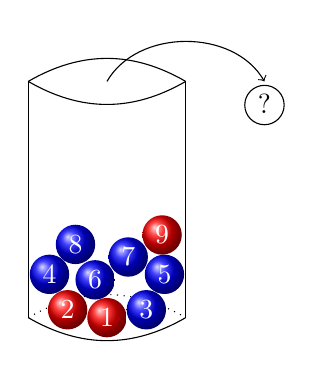
\begin{tikzpicture}
		\draw (0,0) -- (0,-3);
		\draw (2,0) -- (2,-3);
		\draw (0,-3) to [bend right] (2,-3);
		\draw[dotted] (0,-3) to [bend left] (2,-3);
		\draw (0,0) to [bend right] (2,0);
		\draw (0,0) to [bend left] (2,0);
		
		\begin{scriptsize}
		\shade [ball color=red] (1,-3) circle (0.25cm);
		\shade [ball color=red] (0.5,-2.9) circle (0.25cm);
		\shade [ball color=blue] (1.5,-2.9) circle (0.25cm);
		\shade [ball color=blue] (0.27,-2.45) circle (0.25cm);
		\shade [ball color=blue] (1.73,-2.45) circle (0.25cm);
		\shade [ball color=blue] (0.85,-2.52) circle (0.25cm);
		\shade [ball color=blue] (1.27,-2.23) circle (0.25cm);
		\shade [ball color=blue] (0.6,-2.07) circle (0.25cm);
		\shade [ball color=red] (1.7,-1.95) circle (0.25cm);
		\end{scriptsize}
		\node[white] at (1,-3) (1) {1};
		\node[white] at (0.5,-2.9) (2) {2};
		\node[white] at (1.5,-2.9) (3) {3};
		\node[white] at (0.27,-2.45) (4) {4};
		\node[white] at (1.73,-2.45) (5) {5};
		\node[white] at (0.85,-2.52) (6) {6};
		\node[white] at (1.27,-2.23) (7) {7};
		\node[white] at (0.6,-2.07) (8) {8};
		\node[white] at (1.7,-1.95) (9) {9};
		
		\draw[->] (1,0) to [bend left=60] (3,0);
		\draw (3,-0.3) circle (0.25cm);
		\node at (3,-0.29) (a) {?};
	\end{tikzpicture}
\end{document}
%	\caption{Verteilung zu \propref{2_2_6}} 
    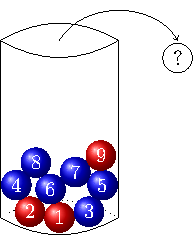
\includegraphics{../../Material/urne_mit_kugeln.pdf}
    \captionof{figure}{Urnenmodell} % needs \usepackage[font=small,labelfont=bf]{caption}
\end{center}

\subsection{Urnenmodell mit Zurücklegen: Multinomial-Verteilung}

Gegeben: Urne mit $N$ Kugeln, verschiedenfarbig mit Farben aus $E$, $\abs{E} \ge 2$ 

Ziehe: $n$ Stichproben/Kugeln, wobei nach jedem Zug die Kugel wieder zurückgelegt wird. Uns interessiert die Farbe in jedem Zug, setze also
\begin{align}
	\Omega = E^n \und \sigF = \pows(\Omega) \notag
\end{align}
Zur Bestimmung einer geeigneten Wahrscheinlichkeitsmaßes, nummerieren wir die Kugeln mit $1,\dots, N$, so dass alle Kugeln der Farbe $a \in E$ eine Nummer aus $F_{a} \subset \set{1,\dots, N}$ tragen. Würden wir die Nummern notieren, so wäre
\begin{align}
	\overline{\Omega} = \set{1,\dots, N}^n \und \overline{\sigF} = \pows(\overline{\Omega})\notag
\end{align}
und wir könnten die Gleichverteilung $\overline{\probp} = \Gleich(\overline{\Omega})$ als Wahrscheinlichkeitsmaß für einem einzelnen Zug verwenden. Für den Übergang zu $\Omega$ konstruieren wir  Zufallsvariablen. Die Farbe im $i$-ten Zug wird beschrieben durch
\begin{align*}
	X_i: \overline{\Omega} \to E \mit \overline{\omega} = \left( \overline{\omega}_1, \dots, \overline{\omega}_n \right) \mapsto a \text{ falls } \overline{\omega}_i \in F_a\\
	\intertext{Der Zufallsvektor}
	X = (X_1, \dots, X_n): \overline{\Omega} \to \Omega\\
   \intertext{beschreibt dann die Abfolge der Farben. Für jedes $\omega \in \Omega$ gilt dann}
	\set{X = \omega} = F_{\omega_1} \times \cdots \times F_{\omega_n} = \bigtimes_{i=1}^{n} F_{\omega_i}\\
	\intertext{und damit}
	\probp(\set{\omega}) 
	&= \overline{\probp}(X^{-1}(\set{\omega})) = \probp(X=\omega)\\
	&= \frac{\abs{F_{\omega_1}} \cdots \abs{F_{\omega_n}}}{\abs{\overline{\Omega}}}\\
	&= \prod_{i=1}^{n} \frac{\abs{F_{\omega_i}}}{N} =: \prod_{i=1}^{n} \rho(\omega_i)
\end{align*}
Zähldichten, die sich als Produkt von Zähldichten schreiben lassen, werden auch als \begriff{Produktdichten} bezeichnet ($\nearrow$  \cref{sec_unabhangigkeit}). %TODO ref?!?!?!

Sehr oft interessiert bei einem Urnenexperiment nicht die Reihenfolge der gezogenen Farben, sondern nur die Anzahl der Kugeln in Farbe $a \in E$ nach $n$ Zügen. Dies enspricht
\begin{align*}
	\hat{\Omega} 
	= \set{k = (k_a)_{a \in E} \in \N_{0}^{\abs{E}} \colon \sum_{a \in E} k_a = n}
	\und \hat{\sigF} = \pows\brackets{\hat{\Omega}}\\
	\intertext{Den Übergang $\Omega \to \hat{\Omega}$ beschreiben wir durch die Zufallsvariablen}
	Y_a(\omega): \Omega \to \N_{0} \mit \omega &= (\omega_1,\dots, \omega_n)\mapsto \sum_{a \in E} \indi_{\set{a}}(\omega_i)\\
	\intertext{und}
	Y = \brackets{Y_a}_{a\in E}: \Omega \to \hat{\Omega} &= \set{k = (k_a)_{a\in E}\colon \sum_{a \in E} k_a = n}
\end{align*}

% % % % % % % % % % % % % % % % % % % % 4th lecture % % % % % % % % % % % % % % % % % % % % % % %

Wir erhalten
\begin{align*}
	\probp(Y = k) &= \probp(Y_a = k_a, \enskip a \in E)\notag\\
	&= \sum_{\omega \in \Omega: Y(\omega) = k} \prod_{i=1}^{n} \rho(\omega_i)\notag\\
	&= \sum_{\omega \in \Omega: Y(\omega) = k} \prod_{a \in E} \rho(a) 
	&= \binom{n}{(k)_{a\in E}} 
%	\begin{pmatrix}
%	n \\
%	(k)_{a\in E}
%	\end{pmatrix}
	\prod_{a \in E} \rho(a)^{k_a},\\
	\intertext{wobei}
	\binom{n}{(k_1, \dots, k_l)} 
	&= 
	\begin{cases}
	\frac{n!}{k_1 ! \, k_2 ! \cdots k_l !} \sum_{i=1}^{l} k_i = n\\
	0 & \sonst
	\end{cases}
\end{align*}
der \begriff{Multinomialkoeffizient} ist, welcher die Anzahl der Möglichkeiten beschreibt, $n$ Objekte in $l$ Gruppen aufzuteilen, so dass Gruppe $i$ gerade $k_i$ Objekte beinhaltet.

\begin{definition}
	Sei $l > 2, p = (p_1, \dots, p_l)$ eine Zähldichte und $n \in \N$, dann heißt die Verteilung auf \\
	$\set{k = (k_i)_{i=1,\dots,l} \in \N_{0}^{l} : \sum_{i=1}^{l} k_i = n}$ mit Zähldichte
	\begin{align}
		m((k_1,\dots,k_l)) = \binom{n}{k_1, \dots, k_l}\prod_{i=1}^{l} p_i^{k_i}\notag
	\end{align}
	\begriff{Multinomialverteilung mit Parametern $n$ und $p$}. Wir schreiben auch $\Multi(n,p)$.
\end{definition}

\begin{example}
	Eine Urne enthalte nur schwarze ``$1$'' und weiße ``$0$'' Kugeln, d.h. $E=\set{0,1}$, und es sei $\rho(1) = p$ gerade die Proportion der schwarzen Kugeln (= Wahrscheinlichkeit bei einem Zug schwarz zu ziehen), dann ist Wahrscheinlichkeit in $n$ Zügen $k$-mal schwarz zu ziehen:
	\begin{align}
		\binom{n}{k}\prod_{i=0,1} \rho(i)^{k_i} = \binom{n}{k} p^k (1-p)^{n-k}.\notag
	\end{align}
	Ein solches (wiederholtes) Experiment mit nur zwei möglichen Ereignissen und fester Wahrscheinlichkeit $p \in [0,1]$ für eines der Ergebnisse nennen wir auch \begriff{(wiederholtes) Bernoulliexperiment}.
\end{example}

\begin{definition}
	Sei $p \in [0,1]$ und $n \in \N$, dann heißt die Verteilung mit Zähldichte
	\begin{align}
		\rho(k) = \binom{n}{k}p^k (1-p)^{n-k} \mit k \in \set{0,1,\dots,n}.\notag
	\end{align}
	\begriff{Binomialverteilung auf $\set{0, \dots,n}$ mit Parameter $p$} (auch \begriff{Erfolgswahrscheinlichkeit}). Wir schreiben auch $\Bin(n,p)$. Im Fall $n = 1$ nennen wir die Verteilung mit Zähldichte
	\begin{align}
		\rho(0) = 1-p \und \rho(1) = p\notag
	\end{align}
	auch \begriff{Bernoulliverteilung mit Parameter $p$} und schreiben $\Ber(p)$.
\end{definition}
\underline{Urnenmodell ohne Zurücklegen}: \begriff{Hypergeometrische Verteilung}\\
Gegeben: Urne mit $N$ Kugeln verschiedener Farben aus $E$,
\begin{align}
	\abs{E} \ge 2.\notag
\end{align}
Es werden $n \le N$ Stichproben entnommen, wobei die gezogenen Kugeln werde \emph{nicht} in die Urne zurückgelegt.

\subsection{Urnenmodell ohne Zurücklegen: Hypergeometrische Verteilung}
Gegeben: Urne mit $N$ Kugeln verschiedener Farben aus $E$, $\abs{E} \ge 2$. Es werden $n \le N$ Stichproben entnommen, wobei die gezogenen Kugeln werde \emph{nicht} in die Urne zurückgelegt.
\begin{example}
	Eine Urne enthalte $S$ schwarze ``$1$'' und $W$ weiße Kugeln ``$0$'' Kugeln, $(E = \set{0,1}, S + W =N)$. Dann ist die Wahrscheinlichkeit in $n$ Zügen ohne Zurücklegen gerade $s$ schwarze und $w$ weiße Kugeln zu ziehen
	\begin{align}
		\rho(w) = \frac{\binom{W}{w}\binom{S}{s}}{\binom{N}{n}}, \quad 0 \le s \le S, 0 \le w \le W, s+w = n, S+W = N.\notag
	\end{align}
\end{example}

\begin{proof}
	Hausaufgabe! %TODO add number later
\end{proof}

\begin{definition}
	Seinen $N \in \N, W \le N, n \le N$, dann heißt die Verteilung auf $\set{0,\dots,n}$ mit Zähldichte
	\begin{align}
		\rho(w) = \frac{\binom{wW}{w}\binom{N-W}{n-w}}{\binom{N}{n}}, \quad w = \max\set{0,n=N+W}, \dots, \min\set{W,n},\notag
	\end{align}
	die \begriff{Hypergeometrische Verteilung} mit Parametern $N,W,n$. Wir schreiben $\Hyper(N,W,n)$.
\end{definition}

\section{Poisson-Approximation und \person{Poisson}-Verteilung}

$\Bin(n,p)$ ist zwar explizit und elementar definiert, jedoch für große $n$ mühsam auszuwerten. Für seltene Ereignisse ($n$ groß, $p$ klein) verwende daher:
\begin{proposition}[Poisson-Approximation]
	Sei $\lambda > 0$ und $(p_n)_{n\in\N}$ eine Folge in $[0,1]$ mit
	\begin{align}
		np_n \to \lambda,\quad n \to \infty.\notag
	\end{align}
	Dann gilt $\forall k \in \N_0$ für die Zähldichte der $\Bin(n,p_n)$-Verteilung
	\begin{align}
		\lim_{n \to \infty} \binom{n}{k}p_n^k(1-p)^{n-k} = e^{-\lambda} \frac{\lambda^k}{k!}.\notag
	\end{align}
\end{proposition}
\begin{proof}
	Sei $k \in \N_{0}$ fix, dann
	\begin{align} %TODO fix this alignment mess and the tags!
		\binom{n}{k} = \frac{n!}{k!(n-k)!} &= \frac{n^k}{k!}\frac{n(n-1)\cdots(n-k+1)}{n^k}\notag\\
		&= \frac{n^k}{k!}\cdot 1 \cdot (1-\frac{1}{n}\cdots \frac{k-1}{n})\notag\\
		\overset{n \to \infty}&{\sim} \frac{n^k}{k!},\notag
	\end{align}
	wobei $a(l) \overset{n \to \infty}{\sim} b(l) \Leftrightarrow \frac{a(l)}{b(l)} \xrightarrow{n\to \infty} 1$. Damit
	\begin{align}
		\binom{n}{k}p^k (1-p)^{n-k} \overset{n \to \infty}&{\sim} \frac{n^k}{k!}p_n^k(1-p_n)^{n-k}\notag\\
		\overset{n \to \infty}&{\sim} \frac{\lambda^k}{k!}(1-p_n)^n\notag\\
		&= \frac{\lambda^n}{k!}\brackets{1 - \frac{np_n}{n}}^n\notag\\
		&\xrightarrow{n \to \infty} \frac{\lambda^n}{k!}e^{-\lambda}.\notag
	\end{align}
\end{proof}
Der erhaltene Grenzwert liefert die Zähldichte auf $\N_{0}$, denn 
\begin{align}
	\sum_{k=0}^{\infty}\frac{\lambda^k}{k!}e^{-\lambda} = e^{-\lambda}\sum_{k=0}^{\infty}\frac{\lambda^{k}}{k!} = e^{-\lambda}e^{\lambda} = 1\notag
\end{align}

\begin{definition}
	Sei $\lambda >0$. Dann heißt das auf $(\N_{0}, \probp(\N_{0}))$ definierte Wahrscheinlichkeitsmaß mit
	\begin{align}
		\probp(\set{k}) = \frac{\lambda^k}{k!}e^{-\lambda} \quad k \in \N_{0},\notag
	\end{align}
	\begriff{Poissonverteilung mit Parameter $\lambda$}. Schreibe $\Pois(\lambda)$.
\end{definition}
Die Poissonverteilung ist ein natürliches Modell für die Anzahl von zufälligen, seltenen Ereignissen (z.B. Tore im Fußballspiel, Schadensfälle einer Versicherung, ...).
\chapter[Bedingte Wkeiten und (Un-)abbhängigkeit]{Bedingte Wahrscheinlichkeiten und (Un-)ab\-hängigkeit}
\chaptermark{Bedingte Wahrscheinlichkeiten und (Un)-abbhängigkeit}
\section{Bedingte Wahrscheinlichkeiten}
\begin{example}
	\proplbl{3_1_1}
	Das Würfeln mit zwei fairen, sechsseitigen Würfeln können wir mit 
	\begin{align}
		\O = \set{(i,j) \colon i,j \in \set{1,\dots,6}}\notag
	\end{align}
	und $\P = \Gleich(\O)$. Da $\abs{\O} = 36$ gilt also
	\begin{align}
		\P(\set{\omega}) = \frac{1}{36} \quad \forall \omega \in \O.\notag
	\end{align}
	Betrachte das Ereignis
	\begin{align}
		A = \set{(i,j) \in \O \colon i + j = 8},\notag
	\end{align}
	dann folgt
	\begin{align}
		\P(A) = \frac{5}{36}.\notag
	\end{align}
	Werden die beiden Würfe nacheinander ausgeführt, so kann nach dem ersten Wurf eine Neubewertung der Wahrscheinlichkeit von $A$ erfolgen.\\
	Ist z.B.
	\begin{align}
		B = \set{(i,j) \in \O, i = 4}\notag
	\end{align}
	eingetreten, so kann die Summe $8$ nur durch eine weitere $4$ realisiert werden, also mit Wahrscheinlichkeit
	\begin{align}
		\frac{1}{6} = \frac{\abs{A \cap B}}{\abs{B}}.\notag 
	\end{align}
	Das Eintreten von $B$ führt also dazu, dass das Wahrscheinlichkeitsmaß $\P$ durch ein neues Wahrscheinlichkeitsmaß $\P_{B}$ ersetzt werden muss. Hierbei sollte gelten:
	\begin{align}
		 &\text{Renormierung: }\P_{B} = 1\label{Renorm}\tag{R}\\
		 &\text{Proportionalität: Für alle} A \subseteq \F \mit A \subseteq B \text{ gilt }
		 \P_{B}(A) = c_B \P(A) \text{ mit einer Konstante } c_B.\label{Prop}\tag{P}
    \end{align}
\end{example}

\begin{lemma}
	Sei $(\O, \F, \P)$ Wahrscheinlichkeitsraum und $B \in \F$ mit $\P(B) > 0$. Dann gibt es genau ein Wahrscheinlichkeitsmaß $\P_B$ auf $(\O, \F)$ mit den Eigenschaften \eqref{Renorm} und \eqref{Prop}. Dieses ist gegeben durch
	\begin{align}
		\P_{B}(A) = \frac{\P(A\cap B)}{\P(B)} \quad \forall A \in \F.\notag
	\end{align}
\end{lemma}

\begin{proof}
	Offenbar erfüllt $\P_{B}$ wie definiert \eqref{Renorm} und \eqref{Prop}. Umgekehrt erfüllt $\P_{B}$ \eqref{Renorm} und \eqref{Prop}. Dann folgt für $A \in \F$:
	\begin{align}
		\P_{B}(A) = \P_{B}(A\cap B) + \underbrace{\P_{B}(A\setminus B)}_{= 0, \text{ wegen } \eqref{Renorm}} \overset{\eqref{Prop}}{=} c_B \P(A \cap B).\notag
	\end{align}
	Für $A=B$ folgt zudem aus \eqref{Renorm}
	\begin{align}
		1 = \P_{B}(B) = c_B \P(B)\notag
	\end{align}
	also $c_B = \P(B)^{-1}$.
\end{proof}

% % % % % % % % % % % % % % % % % % % % % % % % % % % 5th lecture % % % % % % % % % % % % % % % % % % % % % % % % % % %

\begin{definition}
	\proplbl{3_1_3}
	Sei $(\O, \F, \P)$ Wahrscheinlichkeitsraum und $B \in \F$ mit $\P(B) > 0$. Dann heißt
	\begin{align*}
		\P(A\mid B) := \frac{\P(A\cap B)}{\P(B)} \mit A\in \F
	\end{align*}
	die \begriff{bedingte Wahrscheinlichkeit von $A$ gegeben $B$}.
	Falls $\P(B) = 0$, setze
	\begin{align*}
		\P(A \mid B) = 0 \qquad \forall A \in \F
	\end{align*}
\end{definition}

\begin{example} %TODO ref
	In der Situation \propref{3_1_1} gilt % 
	\begin{align*}
		A \cap B = \set{(4,4)}
		\intertext{und damit}
		\P(A \mid B) = \frac{\P(A\cap B)}{\P(B)} = \frac{\frac{1}{36}}{\frac{1}{6}} = \frac{1}{6}
	\end{align*}
\end{example}

Aus \propref{3_1_3} ergibt sich
\begin{lemma}[Multiplikationsformel]
	\proplbl{3_1_4}
	Sei $(\O, \F, \P)$ ein Wahrscheinlichkeitsraum und $A_1, \dots, A_n \in \F$. Dann gilt
	\begin{align*}
		\P(A_1 \cap \cdots \cap A_n) = \P(A_1) \P(A_2 \mid A_1) \dots \P(A_n \mid A_1 \cap \cdots \cap A_{n-1})
	\end{align*}
\end{lemma}

\begin{proof}
	Ist $\P(A_1 \cap \dots \cap A_n) = 0$, so gilt auch $\P(A_n \mid \bigcap_{i=1}^{n-1} A_i) = 0$. Andernfalls sind alle Faktoren der rechten Seite ungleich Null und
	\begin{align*}
		\P(A_1) \P(A_2 \mid A_1) \dots \P(A_n \mid \bigcap_{i=1}^{n-1} A_i) \\
		&= \P(A_1) \cdot \frac{\P(A_1 \cap A_2)}{\P(A_1)} \dots \frac{\P(\bigcap_{i=1}^{n} A_i)}{\P(\bigcap_{i=1}^{n-1}A_i)} \\
		&= \P(\bigcap_{i=1}^n A_i)	
	\end{align*}
\end{proof} %TODO add ref.

Stehen die $A_i$ in \propref{3_1_4} in einer (zeitlichen) Abfolge, so liefert Formel einen Hinweis wie Wahrscheinlichkeitsmaße für \begriff{Stufenexperimente} konstruiert werden können. Ein \emph{Stufenexperiment} aus $n$ nacheinander ausgeführten Teilexperimenten lässt sich als \begriff{Baumdiagramm} darstellen.

%(done) Baumdiagramm
\begin{center}
		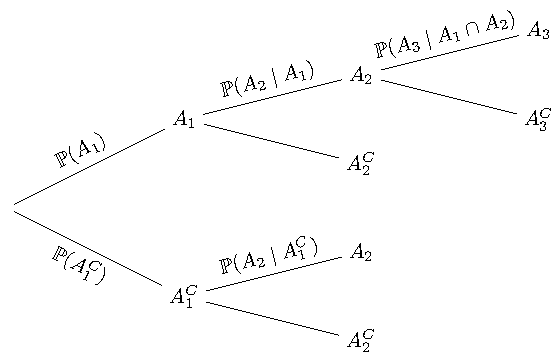
\includegraphics{./tikz/baum_1.pdf}
		\captionof{figure}{\cref{3_1_4}} %\propref{3_1_4}} funktioniert nicht
\end{center}

\begin{proposition}[Konstruktion des Wahrscheinlichkeitsmaßes eines Stufenexperiments]
	\proplbl{3_1_6}
	Gegeben seinen $n$ Ergebnisräume $\O_i = \set{\omega_i (1), \dots, \omega_i (k)}, k \in \N \cup \set{\infty}$ und es sei $\O = \bigtimes_{i = 1}^n \O_i$ der zugehörige Produktraum. Weiter seinen $\F_i$ $\sigma$-Algebren auf $\O_i$ und $\F = \bigotimes_{i=1}^n \F_i$ die Produkt-$\sigma$-Algebra auf $\O$. Setze $\omega = (\omega_1,\dots,\omega_n)$ und
	\begin{align*}
		[\omega_1,\dots,\omega_m]:= \set{\omega_1}\times \dots \times \set{\omega_m} \times \O_{m+1} \times \cdots \times \O_{n},\quad m\le n\\
		\P(\set{\omega_m}[\omega_1,\dots,\omega_{m-1}])
	\end{align*}
	für die Wahrscheinlichkeit in der $m$-ten Stufe des Experiments $\omega_m$ zu beobachten, falls in den vorausgehenden Stufen $\omega_1,\dots,\omega_{m-1}$ beobachten wurden. Dann definiert
	\begin{align*}
		\P(\set{\omega}) := \P(\set{\omega_1}) \prod_{m=2}^{n}\P\brackets{\set{\omega_m} \mid [\omega_1, \dots, \omega_{m-1}]}
		%(done) maybe wrong here. check
	\end{align*}
	ein Wahrscheinlichkeitsmaß auf $(\O, \F, \P)$.
\end{proposition}
\begin{proof}
	Nachrechnen!
\end{proof}

\begin{example}[\person{Polya}-Urne]
	Gegeben sei eine Urne mit $s$ schwarzen und $w$ weißen Kugeln. Bei jedem Zug wird die  gezogene Kugel zusammen mit $c\in \N_0 \cup \set{-1}$ weiteren Kugeln derselben Farbe zurückgelegt.
	\begin{itemize} %TODO seen both in chapter 2.2, but big bracket behind.
		\item $c=0$: Urnenmodell mit Zurücklegen
		\item $c=-1$: Urnenmodell ohne Zurücklegen
	\end{itemize}
	Beide haben wir schon in Kapitel 2.2 gesehen.\\
	Sei deshalb $c\in \N$. (Modell für zwei konkurrierende Populationen) Ziehen wir $n$-mal, so haben wir ein $n$-Stufenexperiment mit 
	\begin{align*}
		\O = \set{0,1}^n \mit \text{ 0 = ``weiß'', 1 = ``schwarz''} \quad (\O_i = \set{0,1})
		\intertext{Zudem gelten im ersten Schritt}
		\P(\set{0}) = \frac{w}{s+w} \und \P(\set{1}) = \frac{s}{s+w}
		\intertext{sowie}
		\P(\set{\omega_m} \mid [\omega_1, \dots \omega_{m-1}]) = 
		\begin{cases} %(done) fix brackets!
		\frac{w+c \brackets{m-1 - \sum_{i=1}^{m-1}\omega_i}}{s+w+c(m-1)} & \omega_m = 0\\
		\frac{s + c\sum_{i=1}^{m-1}\omega_i}{s+w+c(m-1)} & \omega_m = 1
		\end{cases}
	\end{align*}
	Mit \propref{3_1_6} folgt als Wahrscheinlichkeitsmaß auf $(\O, \pows(\O))$
	\begin{align*}
		\P(\set{(\omega_1, \dots, \omega_n)}) &= \P(\set{\omega_1}) \prod_{m=2}^n \P(\set{\omega_m}\mid [\omega_1,\dots,\omega_{m-1}]) \\
		&=\frac{\prod_{i=0}^{l-1}(s+c \cdot i)\prod_{i=0}^{n-l-1}(w + c \cdot j)}{\prod_{i=0}^n (s+w+c \cdot i)} \mit l=\sum_{i=1}^n \omega_i.
		\intertext{Definiere wir nun die Zufallsvariable}
		S_n:\O &\to \N_0 \mit (\omega_1, \dots, \omega_n) \mapsto \sum_{i=1}^n \omega_i
		\intertext{welche die Anzahl der gezogenen schwarzen Kugeln modelliert, so folgt}
		\P(S_n = l) &= \binom{n}{l} \frac{\prod_{i=0}^{l-1}(s+c \cdot i) \prod_{j=0}^{n-l-1}(w + c \cdot j)}{\prod_{i=0}^n(s+w+c \cdot i)}
		\intertext{Mittels $a:= \sfrac{s}{c},b:= \sfrac{w}{c}$ folgt}
		\P(S_n = l) &= \binom{n}{l} \frac{\prod_{i=0}^{l-1}(-a-i)\prod_{j=0}^{n-l-1}(-b-j)}{\prod_{i=0}^n (-a-b-i)} = \frac{\binom{-a}{l}\binom{-b}{n \cdot l}}{\binom{-a-b}{n}}\\ &\mit l \in \set{0,\dots,n} 
	\end{align*}
	Dies ist die \begriff{\person{Polya}-Verteilung} auf $\set{0,\dots,n}, n \in \N$ mit Parametern $a,b > 0$.
\end{example}

\begin{example}
	Ein Student beantwortet eine Multiple-Choice-Frage mit 4 Antwortmöglichkeiten, eine davon ist richtig. Er kennt die richtige Antwort mit Wahrscheinlichkeit $\sfrac{2}{3}$. Wenn er diese kennt, so wählt er diese aus. Andernfalls wählt er zufällig (gleichverteilt) eine Antwort. Betrachte
	\begin{align*}
		W &= \set{\text{richtige Antwort gewusst}}\\
		R &= \set{\text{Richtige Antwort gewählt}}
		\intertext{Dann gilt}
		\P(W) &= \frac{2}{3}, \P(R \mid W) = 1, \P(R \mid W^C) = \frac{1}{4} 
	\end{align*}
	Angenommen, der Student gibt die richtige Antwort. Mit welcher Wahrscheinlichkeit hat er diese gewusst? $\longrightarrow \P(W\mid R) = \text{ ?}$
\end{example}

\begin{proposition}
	\proplbl{3_1_9}
	Sei $(\O, \F, \P)$ Wahrscheinlichkeitsraum und $\O = \bigcup_{i \in I} B_i$ eine höchstens abzählbare Zerlegung in paarweise disjunkte Ereignisse $B_i \in \F$.
	\begin{enumerate} %TODO set itemize references. or use enumerate?
		\item \emph{Satz von der totalen Wahrscheinlichkeit:} Für alle $A \in \F$ gilt
		\begin{align*}
			\P(A) = \sum_{i\in I} \P(A\mid B_i)\P(B_i) \label{eq:totWkeit}\tag{totale Wahrscheinlichkeit}
		\end{align*} 
		\item \emph{Satz von \person{Bayes}:} Für alle $A \in \F$ mit $\P(A) > 0$ und alle $k \in I$
		\begin{align*}
			\P(B_k \mid A) = \frac{\P(A \mid B_k) \P(B_k)}{\sum_{i\in I}\P(A\mid B_i)\P(B_i)} \label{eq:bayes}\tag{Bayes}
		\end{align*}
	\end{enumerate}
\end{proposition}

\begin{proof}
	\begin{enumerate}
		\item Es gilt:
		\begin{align*}
			\sum_{i\in I} \P(A\mid B_i)\P(B_i) \defeq \sum_{i\in I}\frac{\P(A \cap B_i)}{\P(B_i)}\P(B_i) = \sum_{i\in I} \P(A \cap B_i) \overset{\sigma-Add.}{=} \P(A)
		\end{align*}
		\item 
		\begin{align*}
			\P(B_k \mid A) \defeq \frac{\P(A \cap B_k)}{\P(A)} \defeq \frac{\P(A \mid B_k)\P(B_k)}{\P(A)}
		\end{align*}
		also folgt (b) aus (a). %TODO add refs
	\end{enumerate}
\end{proof}

\begin{example}
	In der Situation von \propref{3_1_3} folgt mit \propref{3_1_9} \eqref{eq:totWkeit}
	\begin{align*}
		\P(R) &= \P(R \mid W)\P(W) + \P(R\mid W^C)\P(W^C)\\
		&= 1 \cdot \frac{2}{3} + \frac{1}{4} \frac{1}{3} = \frac{3}{4}
		\intertext{und mit \propref{3_1_9} \eqref{eq:bayes}} %Bayes
		\P(W \mid R) &= \frac{\P(R \mid W)\P(W)}{\P(R)} = \frac{1 \cdot \frac{2}{3}}{\frac{3}{4}} = \frac{8}{9} \text{ für die gesuchte Wahrscheinlichkeit.}
	\end{align*} %(done) compile as pdf and include it. not working.
	\begin{center}
			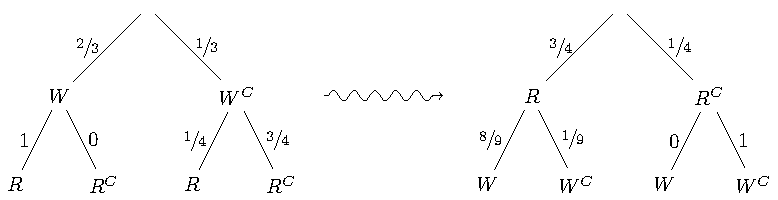
\includegraphics{./tikz/baum_2.pdf}
			\captionof{figure}{\cref{3_1_3}} %\propref{3_1_3} funktioniert nicht
	\end{center}
\end{example}
\section{(Un)abhängigkeit} \label{sec:unabhangigkeit}
In vielen Fällen besagt die Intuition über verschiedene Zufallsexperimente / Ereignisse, dass diese sich \emph{nicht} gegenseitig beeinflussen. Für solche $A,B \in \F$ mit $\P(A) > 0, \P(B) > 0$ sollte gelten
\begin{align*}
\P(A\mid B) = \P(A), \quad \P(B\mid A) = \P(B).
\end{align*}

\begin{definition}[(Stochastische) Unabhängigkeit]
	\proplbl{3_2_11}
	Sei $(\O, \F, \P)$ Wahrscheinlichkeitsraum. Zwei Ereignisse $A,B \in \F$ heißt \begriff{(stochastisch) unabhängig bezüglich $\P$}, falls
	\begin{align*}
		\P(A\cap B) = \P(A)\P(B).
	\end{align*}
	Wir schreiben auch $A \upmodels B$.
\end{definition}
\begin{example}
	Würfeln mit 2 fairen, sechsseitigen Würfeln:
	\begin{align*}
	\O &= \set{(i,j) \mid i,j \in\set{1,\dots,n}},\quad \F = \pows(\O), \quad \P = \Gleich(\O)
	\intertext{Betrachte}
	A:= \set{(i,j) \in \O, i \text{ gerade}}\\
	B:= \set{(i,j) \in \O, j \le 2}.
	\end{align*}
	In diesem Fall, erwarten wir intuitiv Unabhängigkeit von $A$ und $B$.\\
	In der Tat ist % start using \P instead of \P!
	\begin{align*}
	\P(A) = \frac{1}{2}, \quad \P(B) = \frac{1}{3} \und \P(A\cap B) = \frac{1}{6}
	\intertext{was}
	\P(A \cap B) = \P(A) \P(B)
	\intertext{erfüllt}
	\end{align*}
	Betrachte nun
	\begin{align*}
	C&:= \set{(i,j) \in \O \mid i + j = 7}\\
	D&:= \set{(i,j) \in \O \mid i = 6}
	\intertext{dann gilt}
	\P(C) = \frac{1}{6}, \quad \P(D) = \frac{1}{6}
	\intertext{und wegen $C \cap D = \set{(6,1)}$ folgt}
	\P(C\cap D) = \frac{1}{36} = \frac{1}{6} \frac{1}{6} = \P(C) \cdot \P(D)
	\end{align*}
	$C$ und $D$ sind also \emph{stochastisch} unabhängig, obwohl eine kausale Abhängigkeit vorliegt!
\end{example}

\begin{definition}[Unabhängigkeit bezüglich $\P$]
	Sei $(\O, \F, \P)$ Wahrscheinlichkeitsraum und $I \neq \emptyset$ endliche Indexmenge. Dann heißt die Familie $(A_i)_{i \in I}$ von Ereignissen in $\F$ \begriff{unabhängig bezüglich $\P$}, falls für alle $J \subseteq I, J \neq \emptyset$ gilt:
	\begin{align*}
		\P\brackets{\bigcap_{i\in J}A_i} = \prod_{i\in J} \P(A_i)
	\end{align*}
	Offensichtlich impliziert die Unabhängigkeit einer Familie die paarweise Unabhängigkeit je zweier Familienmitglieder nach \propref{3_2_11}. Umgekehrt gilt dies nicht!
\end{definition}

\begin{example}[Abhängigkeit trotz paarweiser Unabhängigkeit]
	Betrachte zweifaches Bernoulliexperiment mit Erfolgswahrscheinlichkeit $\sfrac{1}{2}$, d.h.
	\begin{align*}
		\O = \set{0,1}^2, \quad \F = \pows(\O), \quad \P = \Gleich(\O)
		\intertext{sowie}
		A &= \set{1}\times \set{0,1} \qquad \text{(Münzwurf: erster Wurf ist Zahl)}\\
		B &= \set{0,1}\times \set{1} \qquad \text{(Münzwurf: zweiter Wurf ist Zahl)}\\
		C &= \set{(0,0), (1,1)} \qquad \text{(beide Würfe haben selbes Ergebnis)}
	\end{align*}
	Dann gelten
	\begin{align*}
		\P(A) = \frac{1}{2} = \P(B) = \P(C)
		\intertext{und}
		\P(A\cap B) = \P(\set{(1,1)}) = \frac{1}{4} = \P(A)\P(B)\\
		\P(A\cap C) = \P(\set{(1,1)}) = \frac{1}{4} = \P(A)\P(C)\\
		\P(B\cap C) = \P(\set{(1,1)}) = \frac{1}{4} = \P(B)\P(C)
	\end{align*}
	also paarweise Unabhängigkeit.\\
	Aber
	\begin{align*}
	\P(A\cap B \cap C) = \P(\set{(1,1)}) = \frac{1}{4} \neq \P(A)\P(B)\P(C)
	\end{align*}
	und $A,B,C$ sind \emph{nicht} stochastisch unabhängig.
\end{example}

\begin{definition}[Unabhängige $\sigma$-Algebren]
	\proplbl{3_2_15}
	% started using \O for \Omega and \E for this special generating set E_i
	Seien $(\O, \F,\P)$ Wahrscheinlichkeitsraum, $I \neq \emptyset$ Indexmenge und $(E_i, \Gen_i)$ Messräume
	\begin{enumerate}
		\item Die Familie $\F_i \subset \F, i \in I$, heißen \begriff{unabhängig}, wenn für die $J \subseteq I, J \neq \emptyset, \abs{J} < \infty$ gilt
		\begin{align*}
			\P\brackets{\bigcap_{i \in J} A_i} = \prod_{i\in J} \P(A_i) \qquad \text{ für beliebige } A_i \in \F_i, i \in J
		\end{align*}
		\item Die Zufallsvariable $X_i: (\O, \F) \to (E_i, \Gen_i), i \in I$, heißen \begriff{unabhängig}, wenn die $\sigma$-Algebren
		\begin{align*}
		\sigma(X_i) = X^{-1}(\Gen_i) = \set{\set{X_i \in F} \colon F \in \Gen_i}, \quad i \in I
		\end{align*}
		unabhängig sind.
	\end{enumerate}
\end{definition}

\begin{lemma}[Zusammenhang der Definitionen]
	\proplbl{3_2_16}
	Sei $(\O,\F,\P)$ Wahrscheinlichkeitsraum, $I \neq \emptyset, A \in \F, i \in I$. 
	Die folgenden Aussagen sind äquivalent:
	\begin{enumerate}
		\item Die Ereignisse $A_i, i \in I$ sind unabhängig. 
		\item Die $\sigma$-Algebren $\sigma(A_i), i \in I$ sind unabhängig.
		\item Die Zufallsvariablen $\indi_{A_i}, i \in I$ sind unabhängig.
	\end{enumerate}
\end{lemma}
\begin{proof} %TODO add ref?
	Da die Unabhängigkeit über endliche Teilemengen definiert ist, können wir oBdA $I = \set{1, \dots, n}$ annehmen. 
	\begin{itemize}
		\item Da $\sigma(\indi_{A_i}) = \sigma(A_i)$ folgt die Äquivalenz von 2. und 3. direkt aus \propref{3_2_15}.
		\item Zudem ist 2. $\to$ 1. klar!
		\item Für 1 $\to$ 2. genügt es zu zeigen, dass
		\begin{align*}
			A_1, \dots, A_n \text{ unabhängig } &\Rightarrow B_1, \dots, B_n \text{ unabhängig mit } B_i \in \set{\emptyset, A_i, A_i^C, \O}.
			\intertext{Rekursiv folgt dies bereits aus}
			A_1,\dots, A_n \text{ unabhängig } &\Rightarrow B_1, A_2, \dots, A_n \text{ unabhängig mit } B_1 \in \set{\emptyset, A_1, A_1^C, \O}.
		\end{align*}
		Für $B_1 \in \set{\emptyset, A_1, \O}$ ist dies klar.\\
		Sei also $B_1 = A_1^C$ und $J \subseteq I, J \neq \emptyset$. Falls $1 \not \in J$, ist nichts zu zeigen. Sei $1 \in J$, dann gilt mit
		\begin{align*}
			A &= \bigcap_{i\in J, i \neq 1} A_i
			\intertext{sicherlich}
			\P\brackets{A_1^C \cap A} &= \P(A \setminus (A_1 \cap A))\\
			&= \P(A) - \P(A_1 \cap A)\\
			&= \prod_{i\in J\setminus \set{1}} \P(A_i) - \prod_{i\in J}(A_i)\\
			&= (1- \P(A_1))\prod_{i\in J\setminus \set{1}} \P(A_i)\\
			&= \P\brackets{A_1^C})\prod_{i\in J\setminus \set{1}} \P(A_i)
		\end{align*} 
	\end{itemize}
\end{proof}
Insbesondere zeigt \propref{3_2_16}, dass wir in einer Familie unabhängiger Ereignisse beliebig viele Ereignisse durch ihr Komplement, $\emptyset$ oder $\O$ ersetzen können, ohne die Unabhängigkeit zu verlieren.
\begin{proposition}
	\proplbl{3_2_17}
	Sei $(\O, \F, \P)$ Wahrscheinlichkeitsraum und $\F_i \subseteq \F, i \in I$, seien $\cap$-stabile Familien von Ereignissen. Dann gilt
	\begin{align*}
	\F_i, i \in I \text{ unabhängig } \iff \sigma(\F_i), i \in I \text{ unabhängig}. 
	\end{align*}
\end{proposition}
\begin{proof}
	oBdA sei $I = \set{1, \dots, n}$ und $\O \in \F_i, i \in I$.
	\begin{itemize}
		\item $\Leftarrow$: trivial, da $\F_i \subseteq \sigma(\F_i)$ und das Weglassen von Mengen erlaubt ist.
		\item $\Rightarrow$: zeigen wir rekursiv
		\begin{enumerate}
			\item Wähle $F_i \in \F_i, i = 2, \dots,n$ und defniere für $F \in \sigma(\F_i)$ die endlichen Maße
			\begin{align*}
				\mu(F) = \P\brackets{ F \cap F_2 \cap \cdots \cap F_n} \und \nu(F) = \P(F) \, \P(F_2) \, \dots \, \P(F_n)
			\end{align*}
			\item Da die Familien $\F_i$ unabhängig sind, gilt
			$\mu\mid_{\F_1} = \nu\mid_{\F_1}$.
			Nach dem Eindeutigkeitssatz für Maße (\propref{1_1_9}) folgt $\mu\mid_{\sigma(\F_1)} = \nu\mid_{\sigma(\F_1)}$ also
			\begin{align*}
				\P\brackets{ F \cap F_2 \cap \cdots \cap F_n} = \P(F) \P(F_2) \dots \P(F_n)
			\end{align*}
			für alle $F \in \sigma(\F_i)$ und $F_i \in \F_i, i = 1, \dots, n$. Da $\O \in \F_i$ für alle $i$ gilt die erhaltene Produktformel für alle Teilemengen $J \subseteq I$.\\
			Also sind
			\begin{align*}
			\sigma(\F_1), \F_2, \dots, \F_n \text{ unabhängig}
			\end{align*}
			\item Wiederholtes Anwenden von $1$ und $2$ liefert den Satz.
		\end{enumerate}
	\end{itemize}
\end{proof}
Mit \propref{3_2_17} folgen:
\begin{conclusion}
	\proplbl{3_2_18}
	Sei $(\O,\F,\P)$ Wahrscheinlichkeitsraum und
	\begin{align*}
		\F_{i,j} \subseteq \F, \quad 1 \le i \le n, 1 \le j \le m(i)
	\end{align*}
	unabhängige, $\cap$-stabile Familien.
	Dann sind auch
	\begin{align*}
		\G_i = \sigma(\F_{i,1}, \dots , \F_{i,m(i)}), \quad 1 \le i \le n
	\end{align*}
	unabhängig.
\end{conclusion}
\begin{conclusion}
	\proplbl{3_2_19}
	Sei $(\O,\F,\P)$ Wahrscheinlichkeitsraum und
	\begin{align*}
		X_{ij}: \O \to E, \quad 1 \le i \le n, 1 \le j \le m(i)
	\end{align*}
	unabhängige Zufallsvariablen. Zudem seien $f_i: E^{m(i)} \to \R$ messbar. Dann sind auch die Zufallsvariablen
	\begin{align*}
		f_i(X_{i,1}, \dots, X_{i,m(i)}), \quad 1 \le i \le n
	\end{align*}
	unabhängig.
\end{conclusion}
\begin{example}
	$X_1, \dots, X_n$ unabhängige reelle Zufallsvariablen. Dann sind auch
	\begin{align*}
	Y_1 = X_1, Y_2 = X_2 + \cdots + X_n
	\end{align*}
	unabhängig.
\end{example}
% % % % % % % % % % % % % % % % % 7th lecture % % % % % % % % % % % % % % % % % % %
\begin{proof}[\propref{3_2_18}]
	OBdA sei $\Omega \in \F_{i,j} \forall i,j$. Dann sind die Familien:
	\begin{align*}
		\F_i^{\cap} := \set{F_{i,1} \cap \dots \cap F_{i,m(i)} \mid F_{i,j} \in \F_{i,j}, 1 \le j \le m(i)}, 1 \le i \le n
	\end{align*}
	$\cap$-stabil, unabhängig und es gilt: $\F_{i,1}, \dots, \F_{i,m(i)} \subseteq \F_i^{\cap}$ ($\nearrow$ HA)! Nach \propref{3_2_17} sind auch $\sigma(\F_i^{\cap})$ unabhängig. Damit folgt die Behauptung, da $\sigma(\F_i^{\cap}) = \G_i$:
	\begin{align*}
		\F_{i,1}, \dots, \F_{i,m(i)} \subseteq \F_i^{\cap} \subseteq \sigma(\F_{i,1}, \dots, \F_{i,m(i)}) = \G_i\\
		\Rightarrow \G = \sigma(\F_{i,1}, \dots, \F_{i,m(i)}) \subseteq \sigma(\F_i^{\cap}) \subseteq \G_i.
	\end{align*}
\end{proof}
\begin{proof}[\propref{3_2_19}]
	Setze $\F_{i,j} = \sigma(X_{i,j})$ und $\G_i = \sigma(\F_{i,1}, \dots, \F_{i,m(i)})$, dann sind nach \propref{3_2_18} die $\G_i, i = 1,\dots,n$ unabhängig. Zudem ist
	\begin{align*}
	Y_i := f_i(X_{i,1}, \dots, X_{i,m(i)})
	\end{align*}
	$\G_i$ messbar, also $\sigma(Y_i) \subseteq \G_i$. Damit erben die $Y_i$ die Unabhängigkeit der $\G_i$.
\end{proof}
\begin{proposition}[Unabhängigkeit von Zufallsvariablen]
	\proplbl{3_2_21}
	$(\O, \F, \P)$ Wahrscheinlichkeitsraum und $X_1, \dots, X_n: (\O,\F) \to (E, \E)$ Zufallsvariablen. Dann sind die folgenden Aussagen äquivalent:
	\begin{enumerate}
		\item $X_1, \dots, X_n$ sind unabhängig \label{prop:unabhZV1}
		\item $\P(X_1 \in A_1, \dots, X_n \in A_n) = \prod_{i=1}^n \P(X_i \in A_i)\quad \forall A_1, \dots, A_n \in \E$. \label{prop:unabhZV2}
		\item Die gemeinsame Verteilung der $X_i$ entspricht dem Produktmaß der einzelnen Verteilungen \label{prop:unabhZV3}
		\begin{align*}
			\P_{X_1, \dots, X_n} = \bigotimes_{i=1}^n \P_{X_i}
		\end{align*}
	\end{enumerate}
\end{proposition}
\begin{proof}
	Per Ringschluss:
	\begin{enumerate} %TODO add labels
		\item[1 $\Rightarrow$ 2:] Seien $A_1, \dots, A_n\in E$ beliebig, dann gilt per Definition
		\begin{align*} % für Rechtecke
			\P_{X_1, \dots, X_n}(A_1 \times \dots \times A_n) &= \P(X_1 \in A_1, \dots, X_n \in A_n)\\
			&= \P\brackets{\bigcap_{i=1}^n \set{X_i \in A_i}}\\
			\overset{\text{unabh}}&{=} \prod_{i=1}^n \P(X_i \in A_i)\\
			&= \prod_{i=1}^n \P_{X_i}(A_i) = \brackets{\bigotimes_{i=1}^n \P_{X_i}} (A_1 \times \dots \times A_n) 
		\end{align*} 
		\item[2 $\Rightarrow$ 3:] Aus der obigen Rechnung sehen wir, dass 2 bereits 3 impliziert für alle Rechtecke: $\bigtimes_{i = 1}^n A_i$. Da die Familie der Rechtecke $\cap$-stabil ist und $\E^{\otimes n}$ erzeugt, folgt die Aussage aus dem Eindeutigkeitssatz für Maße \propref{1_1_9}.
		\item[3 $\Rightarrow$ 1:] Sei $J \subseteq \set{1,\dots,n}$ und setze
		\begin{align*}
			A_i &:= \begin{cases}
			\text{ beliebig }  &\text{ in }\E, i \in J\\
			E & i \notin J.
			\end{cases}
			\intertext{Dann}
			\P(X_i \in A_i, i \in J) &= \P(X_i \in A_i, i = 1, \dots,n)\\
			&= \prod_{i=1}^n \P(X_i \in A_i)\\
			&= \prod_{i\in J} \P(A_i \in A_i).
		\end{align*}
	\end{enumerate}
\end{proof}
\begin{example}
	Im Urnenmodell mit Zurücklegen hat der Vektor $X = (X_1, \dots, X_n)$ mit $X_i = $ Farbe im $i$-ten Zug als Zähldichte die Produktdichte der $X_i$. Die $X_1, \dots, X_n$ sind also unabhängig.
\end{example}
\subsection*{Konstruktion unabhängiger Zufallsvariablen}
Kapitel \ref{chapter1}: Zu beliebiger Wahrscheinlichkeitsverteilung $\P_X$ existiert Wahrscheinlichkeitsraum mit Zufallsvariable $X$ auf diesem Wahrscheinlichkeitsraum, so dass $X \sim \P_X$.
\begin{enumerate}
	\item Seien $\P_{X_1}, \dots, \P_{X_n}$ Wahrscheinlichkeitsverteilungen auf $(E, \E)$. Gibt es einen Wahrscheinlichkeitsraum $(\O, \F, \P)$ und Zufallsvariablen $X_1, X_2$ unabhängig, so dass $X_1 \sim \P_{X_1}$? \label{konstruktionunabh:ZV:qu_1}
	\item Wie kann ich beliebig (unendlich) viele unabhängige Zufallsvariablen konstruieren? \label{konstruktionunabh:ZV:qu_2}
\end{enumerate}
Wir beginnen mit \ref{konstruktionunabh:ZV:qu_1}:\\
Konstruiere zwei Wahrscheinlichkeitsräume $(\O_i, \F_i, \P_i), i = 1,2$ und Zufallsvariablen $X_1, X_2 \mit X_i \sim \P_{X_i}$. Auf dem Produktraum
\begin{align*}
	\O = \O_1 \times \O_2, \quad \F := \F_1 \otimes \F_2 \und \P = \P_1 \otimes \P_2
	\intertext{ definiere}
	X'_1: \O_1 \times \O_2 \to E\colon (\omega_1, \omega_2) \mapsto X_1(\omega_1)\\
	X'_2: \O_1 \times \O_2 \to E\colon (\omega_1, \omega_2) \mapsto X_2(\omega_2)
\end{align*}
Dann gilt für beliebige Ereignisse: $F_1, F_2 \in \E$
\begin{align*}
	\underbrace{\set{X'_1 \in F_1} \cap \set{X'_2 \in F_2}}_{\supseteq \O = \O_1 \times \O_2} = \underbrace{\set{X_1 \in F_1}}_{\supseteq \O_1} \times \underbrace{\set{X_2 \in F_2}}_{\supseteq \O_2} \in \F_1 \times \F_2
\end{align*}
und damit folgt die Messbarkeit der Abbildungen $X'_1, X'_2$, d.h. $X'_1, X'_2$ sind Zufallsvariablen auf $(\O, \F)$. Zudem gilt
\begin{align*}
	\P(X'_1 \in F_1, X'_2 \in F_2) &= \P_1 \otimes \P_2 \brackets{\set{X_1 \in F_1} \times \set{X_2 \in F_2}}\\
	&= \P_1 (X_1 \in F_1) \P_2(X_2 \in F_2),
	\intertext{also}
	\P(X'_i \in F_i) &= \P_i (X'_i \in F_i)
\end{align*}
sowie nach \propref{prop:Kolmo} $X'_1 \upmodels X'_2$.\\
Wenn $(\O_2, \F_1, \P_1) = (\O_2, \F_2, \P_2)$, so liefert die obige Konstruktion zwei unabhängige Zufallsvariablen auf einem Wahrscheinlichkeitsraum. Andernfalls können wir auf den Produktraum ausweichen und $X'_i$ anstelle von $X_i$ betrachten. Die obige Konstruktion lässt sich direkt auf \emph{endlich} viele Zufallsvariablen übertragen.\\
Zu \ref{konstruktionunabh:ZV:qu_2}: 
\begin{proposition}[Satz von \person{Kolmogorov}]
	\proplbl{prop:Kolmo}
	Sei $I$ beliebige Indexmenge und $(\O_i, \F_i, \P_i), i \in I$ Wahrscheinlichkeitsräume. Setze
	\begin{align*}
		\O_I &:= \bigtimes_{i \in I} \O_i = \set{\omega : I \to \bigcup_{i \in I} \O_i, \omega_i \in \O_i, i \in I}\\
		\F_I &:= \sigma( \pi^{-1} ( \F_i), i \in I)
	\end{align*}
	wobei $\pi_i : \O_I \to \O_i \mit \omega \longmapsto \omega_i$ die Projektionsabbildung. Dann existiert auf $(\O_I, \F_I)$ genau ein Maß $\P_I$, sodass für alle $H \subseteq I$ mit $0 < \abs{H} < \infty$ gilt
	\begin{align*}
		\pi_H ( \P_I) = \bigotimes_{i \in H} \P_i,
	\end{align*}
	wobei $\pi_H: \O_I \to \O_H$ wiederum die Projektionsabbildung.
\end{proposition}
\begin{proof}
	$\nearrow$ Schilling Maß und Integral, Satz 17.4.
\end{proof}
Sind auf den Wahrscheinlichkeitsräumen $(\O_i , \F_i , \P_i), i \in I$, nun Zufallsvariablen $X_i: \O_i \to E$ gegeben, so definieren wir wie im Satz von Kolmogorov (\propref{prop:Kolmo})
\begin{align*}
	(\O, \F, \P) := \brackets{\O_I, \F_I, \P_I = \bigotimes_{i \in I}} \mit \omega = (\omega_i)_{i \in I}
	\intertext{und wie im endlichen Fall}
	X'_i : \O \to E \mit X'_i (\omega) = X_i (\omega_i).
\end{align*}
Da die Unabhängigkeit der Zufallsvariablen über endliche Teilfamilien definiert ist, folgt diese wie im endlichen Fall. 
\subsection*{Faltungen}
Seien $X, Y$ zwei reelle und unabhängige Zufallsvariablen mit 
\begin{align*}
	X \sim \P_X \und Y \sim \P_Y.
\end{align*}
Dann hat $(X,Y)$ die Verteilung $\P_X \otimes \P_Y$ auf $\R^2$. Andernfalls ist auch $X+Y$ eine reelle Zufallsvariable, dann
\begin{align*}
	X + Y = A(X,Y) \mit A: \R^2 \to \R: (x,y) \mapsto x + y.
\end{align*}
$A$ ist stetig, also messbar. Die Verteilung von $X+Y$ ist dann $(\P_X \otimes \P_Y)\circ A^{-1}$.
\begin{definition}[Faltung]
	\proplbl{3_2_24}
	Seien $\P_1 , \P_2$ Wahrscheinlichkeitsmaße auf $(\Rn, \borel(\Rn))$. Das durch
	\begin{align*}
		\P_1 \star \P_2(F) = \iint \indi_F (x+y) \P_1 (\d x)\P_2 (\d y)
	\end{align*}
	definierte Wahrscheinlichkeitsmaß $\P_1 \ast \P_2 = (\P_1 \otimes \P_2) \circ A^{-1}$ auf $(\Rn, \borel(\Rn))$ heißt \begriff{Faltung} von $\P_1$ und $\P_2$.
\end{definition}
\begin{proposition}
	\proplbl{3_2_25}
	Seien $X,Y: \O \to \Rn$ unabhängige Zufallsvariablen mit Verteilungen $\P_X, \P_Y$. Dann ist
	\begin{align*}
		\P_{X+Y} = \P_X \star \P_Y,
	\end{align*}
	die Verteilung von $X +  Y$.
\end{proposition}
\begin{proof}
	Siehe Herleitung Faltung.
\end{proof}
Faltung von Wahrscheinlichkeitsmaßen und Dichten besitzen wieder eine Dichte.
\begin{proposition}
	\proplbl{3_2_26}
	Seien $\P_1 , \P_2$ Wahrscheinlichkeitsmaße auf $(\R, \borel(\Rn))$
	\begin{enumerate}
		\item Diskreter Fall: Sind $\P_1 , \P_2$ de facto Wahrscheinlichkeitsmaße auf $(\Z, \pows(\Z))$ mit Zähldichte $\rho_1 , \rho_2$. Dann ist die Faltung $\P_1 \star \P_2$ Wahrscheinlichkeitsmaß auf $(\Z, \borel(\Z))$ mit Zähldichte
		\begin{align*}
			\rho_1 \star \rho_2 (k) = \sum_{l \in \Z} \rho_1 (l) \rho_2 (k-l).
		\end{align*}
		\item Stetiger Fall: Besitzt $\P_1 , \P_2$ Dichtefunktionen $\rho_1, \rho_2$, so besitzt die Faltung $\P_1 \star \P_2$ die Dichtefunktion
		\begin{align*}
			\rho_1 \star \rho_2 (x) = \int_{\R} \rho_1 (y) \rho_2 (x-y) \d y \quad x \in \R
		\end{align*}
	\end{enumerate}
\end{proposition}
\begin{proof}
	\begin{enumerate}
		\item Diskrete Fall: Sei $k \in \Z$
		\begin{align*}
			(\P_1 \otimes \P_2)(A = k) &= \sum_{\substack{l_1,l_2 \in \Z\\ l_1 + l_2 = k}} \rho_1 (l_1) \rho_2 (l_2)\\
			&= \rho_1 \star \rho_2 (k)
		\end{align*}
		\item Stetiger Fall: Sei $c \in \R$ 
		\begin{align*}
		\P_1 + \P_2 ((-\infty, c]) &= (\P_1 \otimes \P_2)(A \le c)\\
		&= \int_{\R}\int_{\R} \indi_{(\infty,c]} (x+y) \rho_1 (x) \rho_2 (y) \d x \d y\\
		\overset{y = z -x}&{=} \int_{\R}\int_{\R} \indi_{(\infty,c]} (z) \rho_1 (x) \rho_2 (z-x) \d x \d z\\
		&= \int_{-\infty}^c \underbrace{\int_{\R} \rho_1 (x) \rho_2 (z-x) \d x}_{\rho_1 \star \rho_2 (z)} \d z.
		\end{align*}
	\end{enumerate}
\end{proof}
\begin{example}
	\proplbl{3_2_27}
	Seien $X \sim \Pois(\lambda), Y \sim \Pois(\mu)$ zwei unabhängigen reellen Zufallsvariablen (mit Werten in $\N_0$). Dann ist $X+Y$ eine Zufallsvariable mit Werten in $\N_0$ und Zähldichte
	\begin{align*}
		\P(X+Y=k) &= \sum_{l \in \Z} \P(X=l) \P(Y = k-l)\\
		&= \sum_{l \in \Z} \frac{\lambda^l}{l!} e^{-\lambda} \frac{\mu^{k-l}}{(k-l)!} e^{-\mu}\\
		&= e^{-(\lambda + \mu)} \frac{1}{k!}\sum_{l=0}^k \binom{k}{l} \lambda^l \mu^{k-l}\\
		&= e^{-(\lambda + \mu)} \frac{1}{k!} (\lambda + \mu)^k \quad \forall k \in \N_0,
		\intertext{so dass}
		X + Y &\sim \Pois(\lambda + \mu).
	\end{align*}
	D.h. der Typ der Verteilung ist bei der Faltung erhalten geblieben.
\end{example}
\begin{*hint}
	Das ist aber nicht immer der Fall!
\end{*hint}
\begin{example}
	\proplbl{3_2_28}
	Seien $X,Y \sim \Gleich([0,1])$ zwei unabhängige Zufallsvariablen mit Dichten $\rho(x) = \indi_{[0,1]}(x)$. Dann ist $X+Y$ eine Zufallsvariable mit Werten in $[0,2]$ und Dichte
	\begin{align*}
		\rho \star \rho(x) &= \int_{\R} \rho(y) \rho(x-y) \d x \d y\\
		&= \int_{\R} \indi_{[0,1]}(y) \indi_{[0,1]}(x-y) \d y\\
		&= \int_{0 \vee (x-1)}^{1 \wedge x} \d y= \begin{cases}
		x &\quad 0 \le x \le 1\\
		2 -x &\quad 1 \le x \le 2\\
		0 &\quad \sonst.
		\end{cases}
	\end{align*} %TODO add pics
%	\begin{tikzpicture}
%	
%	\end{tikzpicture}
%	\begin{tikzpicture}
%	
%	\end{tikzpicture}
\end{example}

\chapter{Weitere Standardmodelle der Wahrscheinlichkeitstheorie}
\section{Stetige Gleichverteilung}
\begin{*erinnerung}
	$\O \subset \Rn$ Borel-messbar mit \person{Lebesgue}volumen $0 < \lambda(\O) < \infty$. Wahrscheinlichkeitsmaß ist $(\O, \borel(\O))$ mit Dichte
	\begin{align*}
	q\rho(x) = \frac{1}{\lambda(\O)}
	\end{align*}
	heißt stetige Gleichverteilung auf $\O$: $\Gleich(\O)$.\\
	Für alle $A \in \borel(\O)$ gilt:
	\begin{align*}
		\P(A) = \int_{A} \rho(x) \d x = \frac{\lambda(A)}{\lambda(\O)}.
	\end{align*}
	Meist verwenden wir $\Gleich([a,b]), a < b$ (Gleichverteilung auf Intervall) mit $\rho(x) = \sfrac{1}{(b-a)}, a \le x \le b$ und Verteilungsfunktion
	\begin{align*}
		F(x) = 
		\begin{cases}
			0 & x < a\\
			\int_{a}^{x} \frac{x-a}{b-a} & a \le x \le b\\
			1 & x >b
		\end{cases}
	\end{align*}
\end{*erinnerung}
\section{Wartezeitverteilungen}
\begriff{Negative Binomialverteilung}:\
Wir wiederholen ein Bernoulliexperiment mit Erfolgswahrscheinlichkeit $p \in [0,1]$ unendlich oft. Gesucht ist die Anzahl der Misserfolge bis zum $r$-ten Erfolg, $r \in \N$. Ein passender Ergebnisraum ist $\O = \N_0$. Für Modellierung ist es jedoch leichter in jedem Versuch Erfolgt (``1'') oder Misserfolg (``0'') festzuhalten und $i$ mit dem unendlichen Produktmaß des Bernoullimaßes auf $\set{0,1}^{\N}$ zu arbeiten.\\
Als Zufallsvariable
\begin{align*}
	X_r : \set{0,1}^{\N} \to \O
\end{align*}
welche die Anzahl der Misserfolge bis zum $r$-ten Erfolg darstellt, setze
\begin{align*}
	X_r (\omega) &= \min \set{\sum_{i=1}^k \omega_i = r} = r
	\intertext{Dann}
	\P(X_r = k) &= \sum_{\substack{\omega \in \set{0,1}^{\N}\\ X_r(\omega) = k}} \prod_{i=1}^{\infty} \rho(\omega_i)
	\intertext{mit $\rho(0) = 1-p, \rho(1) = 1$ (Zähldichte der Bernoulliverteilung), also}
	\P(X_r = k) &= \binom{r+k-1}{k} (1-p)^k p^r \quad r \in \N_0.
\end{align*}
\begin{definition}[negative Binomialverteilung, geometrische Verteilung]
	Sei $p \in[0,1]$ und $r \in \N$, dann heißt die Verteilung auf $\N_0$ mit Zähldichte
	\begin{align*}
		\rho(k) = \binom{r+k-1}{k} p^r (1-p)^k
	\end{align*}
	\begriff{negative Binomialverteilung} mit Parametern $(r,p)$. Schreibe $\negBin(r,p)$. Im Fall $r = 1$ nennen wir die Verteilung mit Zähldichte
	\begin{align*}
		\rho(k) = p(1-p)^k \quad k \in \N_0
	\end{align*}
	\begriff{geometrische Verteilung} mit Parametern $p$. Schreibe $\Geom(p)$.
\end{definition}
\section{Wartezeitverteilungen}

\emph{Negative Binomialverteilung}:\\
Wir wiederholen ein Bernoulliexperiment mit Erfolgswahrscheinlichkeit $p \in [0,1]$ unendlich oft. Gesucht ist die Anzahl der Misserfolge bis zum $r$-ten Erfolg, $r \in \N$. Ein passender Ergebnisraum ist $\O = \N_0$. Für Modellierung ist es jedoch leichter in jedem Versuch erfolgt (``1'') oder Misserfolg (``0'') festzuhalten und $i$ mit dem unendlichen Produktmaß des Bernoullimaßes auf $\set{0,1}^{\N}$ zu arbeiten.\\
Als Zufallsvariable
\begin{align*}
	X_r : \set{0,1}^{\N} \to \O
\end{align*}
welche die Anzahl der Misserfolge bis zum $r$-ten Erfolg darstellt, setze
\begin{align*}
	X_r (\omega) &= \min \set{\sum_{i=1}^k \omega_i = r} = r.
	\intertext{Dann}
	\P(X_r = k) &= \sum_{\substack{\omega \in \set{0,1}^{\N}\\ X_r(\omega) = k}} \prod_{i=1}^{\infty} \rho(\omega_i)
	\intertext{mit $\rho(0) = 1-p, \rho(1) = 1$ (Zähldichte der Bernoulliverteilung), also}
	\P(X_r = k) &= \binom{r+k-1}{k} (1-p)^k p^r \quad r \in \N_0.
\end{align*}
\begin{definition}[negative Binomialverteilung, geometrische Verteilung]
	Sei $p \in[0,1]$ und $r \in \N$, dann heißt die Verteilung auf $\N_0$ mit Zähldichte
	\begin{align*}
		\rho(k) = \binom{r+k-1}{k} p^r (1-p)^k
	\end{align*}
	die \begriff{negative Binomialverteilung} mit Parametern $(r,p)$. Schreibe $\negBin(r,p)$. Im Fall $r = 1$ nennen wir die Verteilung mit Zähldichte
	\begin{align*}
		\rho(k) = p(1-p)^k \quad k \in \N_0
	\end{align*}
	\begriff{geometrische Verteilung} mit Parametern $p$. Schreibe $\Geom(p)$.
\end{definition}

\subsection{Exponential- und Gammaverteilung}

\begin{enumerate}
	\item \emph{Ziel:} Modelliere die Wartezeit auf $r$ Ereignisse in kontinuierlicher Zeit.
	\item \emph{Wähle:} $(\Omega, \F) = (\R_+, \borel(R_+))$
	\item \emph{Annahmen:} 
	\begin{itemize}
		\item Jedes Ereignis geschieht zu einer zufälligen Zeit
		\item Die Anzahl der Ereignisse bis zur Zeit $t$ sei $\Pois(\lambda t)$ verteilt.
	\end{itemize}
	Die zweite Annahme macht Sinn, denn
	\begin{itemize}
		\item Poissonverteilung ist Modell für Anzahl seltener Ereignisse
		\item Nach Beispiel 3.26:
		\begin{align*}
			\Pois(\lambda t) \star \Pois(\lambda s) = \Pois(\lambda(t+s)) 
		\end{align*}
		Die Linearität des Parameters entspricht also einer Stationaritätsvorrausetzung:\\
		Modelliert
		\begin{align*}
			X\sim\Pois(\lambda t) \text{ die Ereignisse in } (0,t],\\
			Y\sim\Pois(\lambda s) \text{ die Ereignisse in } (t,t+s]
			\intertext{so modelliert}
			X+Y \sim \Pois(\lambda (t+s)) \text{ die Ereignisse in } (0,t+s].
		\end{align*}
	\end{itemize}
\end{enumerate}
Unter diesen Annahmen folgt für die Wahrscheinlichkeit in $(0,t]$ mindestens $r$ Ereignisse zu beobachten
\begin{align*}
	\P ((0,t)) &= 1-\sum_{k=0}^{r-1} \underbrace{e^{-\lambda t} \frac{(\lambda t)^k}{k!}}_{\text{Zähldichte }\Pois(\lambda t)\text{ in }t}  \\
	\frac{\d}{\d t} &\brackets{1- \sum_{k=0}^{r-1} e^{-\lambda t} \frac{(\lambda t)^k}{k!}}  \\
	&= - (-\lambda) e^{-\lambda t} \sum_{k=0}^{r-1} \frac{(\lambda t)^k}{k!} - e^{-\lambda t} \sum_{k=0}^{r-1} \frac{\lambda^k t^{k-1}}{(k-1)!}  \\
	&= e^{-\lambda t} \left(\sum_{k=0}^{r-1} \frac{\lambda^k t^{k-1}}{k!} - \sum_{l=0}^{r-1} \frac{\lambda^k t^{l-1}}{(l-1)!}\right) 
\end{align*}
gilt
\begin{align*}
	\P((0,t)) = \int_{0}^t e^{-\lambda t} \frac{\lambda^r x^{r-1}}{(r-1)!} \d x.
\end{align*}

Wir definieren allgemeiner:
\begin{definition}[Gammaverteilung, Gammafunktion]
	Seinen $\lambda > 0, r>0$, dann heißt die Verteilung auf $(\R_+, \borel(\R_+))$ mit Dichte
	\begin{align*}
		f(x) = \frac{\lambda^r}{\Gamma(r)} x^{r-1} e^{-\lambda x},
		\intertext{wobei}
		\Gamma(r) = \int_{0}^{\infty} y^{r-1}e^{-y} \d y, r>0
	\end{align*}
	\begriff{Gammefunktion}, \begriff{Gammaverteilung} mit Parametern $\lambda,r$. Schreibe $\Gam(\lambda,r)$.
\end{definition}
Insbesondere ist $\Geom(\lambda,1)$ gerade die \begriff{Exponentialverteilung} (vgl. Bsp 17?).\\ %TODO add ref?
Die Gammaverteilung ist reproduktiv: Die Wartezeit auf $r+s$ Ereignisse entspricht der Wartezeit auf $r$ Ereignisse + $s$ (weitere) Ereignisse:
\begin{lemma} % lemma 4.4
	Seien $X \sim \Gam(\lambda,r), Y \sim \Gam(\lambda,s)$ unabhängig, dann impliziert das
	\begin{align*}
		X+Y \sim \Gam(\lambda,r+s)
	\end{align*}
\end{lemma}
\begin{proof}
	Hier nur für $r,s \in \N$, allgemein später mit \begriff{momenterzeugende Funktionen}.\\
	Seien $\rho(x), \rho(y)$ Dichten von $X,Y$. Nach \propref{3_2_25} folgt
\begin{align*}
	\rho_{(X+Y)} &= \rho_X \star \rho_Y (x) = \int_{\R} \rho_X(y)\rho_Y(x-y) \d y  \\
	&= \int_{\R} \frac{\lambda^r}{\Gamma(r)} y^{r-1} e^{-\lambda y} \frac{\lambda^s}{\Gamma(s)} (x-y)^{s-1} e^{-\lambda (x-y)} \d y  \\
	&= \frac{\lambda^{r+s}}{\Gamma(r)\Gamma(s)} e^{-\lambda x} \int_0^x y^{r-1} (x-y)^{s-1} \d y  \\
	\over{\text{part Int}}&{=} \frac{\lambda^{r+s}}{\Gamma(r)\Gamma(s)} e^{-\lambda x} \brackets{\underbrace{\left[\frac{1}{r} y^r (x-y)^{s-1}\right]_{y=0}^x}_{=0} + \frac{s-1}{r} \int_0^x y^r (x-y)^{s-2} \diff y }  \\
	\over{\text{Ind}}&{=} \frac{\lambda^{r+s}}{\Gamma(r)\Gamma(r)} e^{-\lambda x} \frac{\Gamma(r)\Gamma(s)}{\Gamma(r+s)} = \frac{\lambda^{r+s}}{\Gamma(r+s)} e^{-\lambda x}. 
\end{align*}
\end{proof}
Exponentialverteilung sind zudem \begriff{gedächnislos}:
\begin{lemma}
	Sei $X \sim \EXP(\lambda)$, dann gilt
	\begin{align*}
		\P(X>t) = \P(X > t+s \mid X > s) \quad t,s \ge 0. \tag{$\ast$}\label{lem:eq:gedachtnislos}
	\end{align*}
\end{lemma}
\begin{proof}
	\begin{align*}
		\P(X > t+s \mid X \ge s) &= \frac{\P(X> t+s, X \ge s)}{\P(X > s)}\\
		&= \frac{\P(X > t+s)}{\P(X > s)}\\
		&= \frac{e^{-\lambda(t+s)}}{e^{-\lambda t}} = e^{-\lambda t} = \P(X> t).
	\end{align*}
\end{proof}
\begin{example}
	\proplbl{4_2_5}
	Eine Studentin wartet morgens eine $\EXP(\sfrac{1}{s})$ verteilte Zeit $X$ auf den Bus zur Uni. Die Wahrscheinlichkeit einer Wartezeit $\ge 5$ Minuten
	\begin{align*}
	\P(X \ge 5) = e^{-\frac{1}{s}} = e^{-1} \approx 0,37.
	\end{align*}
	An einen kalten, stürmischen Frühlingstag hat die Studentin bereits 10 Minuten gewartet. Die Wahrscheinlichkeit mindestens 5 weitere Minuten zu warten ist
	\begin{align*}
	\P(X\ge 15 \mid X > 10) = \P(X\ge 5) = e^{-1} \approx 0,37.
	\end{align*}
\end{example}
\begin{*hint}
	Man kann sogar zeigen, dass die Exponentialverteilung die einzige absolutstetige Verteilung mit \eqref{lem:eq:gedachtnislos} ist.
\end{*hint}
\chapter{Erwartungswerte \& Varianz}
\begin{enumerate}
	\item \emph{Frage:} \\
	\cref{4_2_5} Durchschnittliche Wartezeit? $\rightsquigarrow$ Erwartungswert\\
	Wie stark ist die Streuung um den Durchschnitt? $\rightsquigarrow$ Varianz
\end{enumerate}
\section{Der Erwartungswert}
\begin{definition}[Erwartungswert]
	\proplbl{5_1_1}
	Sei $(\O, \F, \P)$ Wahrscheinlichkeitsraum und $X: (\O, \F) \to (\R, \borel(\R))$ Zufallsvariable. Dann ist
	\begin{align*}
		\E[X] = \int_{\O} X(\omega) \P(\d \omega) = \int_{\R} x \P(X  \in \d x)
	\end{align*}
	der \begriff{Erwartungswert von $X$}.
\end{definition}
\begin{*hint}
	Der Erwartungswert von $X$ existiert, genau dann wenn
	\begin{align*}
		\int_{\O} \abs{X(\omega)}\P(\d \omega) < \infty \bzw \E[\abs{X}] < \infty
	\end{align*}
	d.h. genau dann wenn $X \in \Ln{1} (\P)$.\\
	Für nichtnegative Zufallsvariablen ist der Erwartungswert immer definiert, wenn wir $+\infty$ als zulässigen Wert annehmen, was wir in der Folge auch tun.
\end{*hint}
\begin{example}
	\proplbl{5_1_2}
	$(\O, \F, \P)$ Wahrscheinlichkeitsraum, $A \in \F$ und sei $X: (\O, \F) \to (\R, \borel(\R))$ die Indikatorvariable %TODO should be X right? (Y-->X)
	\[
		X(\omega) = \indi_{A} (\omega)
	\]
	Dann gilt: $X \in \Ln{1}(\P)$ und
	\begin{align*}
		\E[X] = \int_{\O} \indi_{A} (\omega) \P(\d \omega) = \int_{A} \P(\d \omega) = \P(A).
	\end{align*}
\end{example}
\begin{proposition}
	\proplbl{5_1_3}
	Sei $X: (\O, \F) \to (\Rn, \borel(\Rn)$ Zufallsvariable und $f: \Rn \to \R$ Borel-messbar. Dann
	\begin{align*}
		\E[f(X)] = \int f(X)\d \P = \int_{\O} \E(X(\omega)) \d \P(\omega) = \int_{\Rn} f(X) \P(X \in \d x). 
	\end{align*}
\end{proposition}
\begin{proof}
	Sei $f(X)$ eine reelle Zufallsvariable. Die Formel folgt direkt auf dem Transformationssatz für Bildmaße ($\nearrow$ Schilling MINT 18.1).
\end{proof}
\begin{proposition}[Erwartungswerte bei Existenz einer (Zähl-)dichte]
	\proplbl{5_1_4}
	Sei $X: (\O, \F) \to (\Rn, \borel(\Rn))$ Zufallsvariable und
	\begin{align*}
		f: \Rn \to \R \text{ Borel-messbar}.
	\end{align*}
	\begin{enumerate}
		\item \emph{diskreter Fall:} Ist $\P_X$ ein Wahrscheinlichkeitsmaß auf $(\Z, \P(\Z))$ und der Zähldichte $\rho$, so
		\begin{align*}
			\E[f(X)] = \sum_{x \in \Z} f(x)\rho(x).
		\end{align*}
		\item \ul{stetiger Fall:} Besitzt $\P_X$ eine Dichte $\rho$ (bzgl Lebesguemaß), so
		\begin{align*}
			\E[f(X)] = \int_{\R} f(x)\rho(x) \d x
		\end{align*}
	\end{enumerate}
\end{proposition}
\begin{proof}
	Klar aus \propref{5_1_1} und \propref{5_1_3}. %TODO ref
\end{proof}
\begin{example}
	\proplbl{5_1_5}
	Sei $X \sim \Bin(n,p)$. Dann gilt
	\begin{align*}
		\E[X] &= \sum_{k=1}^n k\binom{n}{k}p^k (1-p)^{n-k}\\
		&= \sum_{k=1}^n \frac{n!}{(n-k)!(k-1)!}p^k (1-p)^{n-k}\\
		&= np \sum_{k=1}^n \underbrace{\binom{n-1}{k-1}p^{k-1}(1-p)^{n-1-(k-1)}}_{\text{Zähldichte }\Bin(n-1,p) \text{ in } k-1}\\
		&= np.
	\end{align*}
\end{example}
Da der Erwartungswert ein Integral ist, übertragen sich viele Eigenschaften. 
\begin{proposition}[Eigenschaften des Erwartungswertes]
	Seien $X,Y,X_n: (\O,\F) \to (\R, \borel(\R)), n \in \N$ Zufallsvariablen in $\Ln{1}(\P)\und a,b \in \R$ konstant.
	\begin{enumerate}
		\item \ul{Linearität:} $\E[aX +bY] = a\E X + b\E Y$
		\item \ul{Monotonie:} $X \le Y$, d.h. $X(\omega) \le Y(\omega), \forall \omega \in \Omega$. Dann gilt 
		\[
			\E[X] \le \E[Y] \text{ und insbesondere gilt } X \ge 0 \implies \E X \ge 0.
		\]
		\item \ul{Lemma von \person{Fatou}:}
		\begin{align*}
			\E[\liminf_{n \to \infty}X_n] \le \liminf_{n \to \infty} \E[X_n]
		\end{align*}
		\item \ul{Satz von \person{Beppo}-\person{Levi}:} Wenn $X_n \ge 0 \und X_n \uparrow X$ so gilt:
		\begin{align*}
			\E[X] = \sup_{n \in \N} \E[X_n] = \lim_{n \to \infty} \E[X_n]
		\end{align*}
		\item \ul{Dominierte Konvergenz/ Satz von \person{Lebesgue}:} Sei $\lim_{n \to \infty} X_n(\omega) = X(\omega)$ und
		\begin{align*}
		\P(\set{\omega: \abs{X_n(\omega)} \le Y(\omega)}) = 1 \qquad (\abs{X} \le Y \P \text{ fast sicher})
		\end{align*}
		für $Y \in \Ln{1}(\P) \implies X \in \Ln{1}(\P) \und \lim_{n \to \infty} \E[X] = \E[X]$
		\item \ul{\person{Markov}-Ungleichung:} Sei $\epsilon > 0$, dann gilt
		\begin{align*}
		\P(\abs{X} \ge \epsilon) \le \frac{1}{\epsilon} \E[\abs{X}]
		\end{align*}
		\item \ul{\person{Hölder}-Ungleichung:} Sei $1 \le p,q = \infty, \frac{1}{p}+ \frac{1}{q} = 1$
		\begin{align*}
		\E[\abs{XY}] \le \brackets{\E[\abs{X}^p]}^{\frac{1}{p}} \brackets{\E[\abs{Y}^q]}^{\frac{1}{q}}
		\end{align*}
		($p =q =2$ \person{Cauchy}-\person{Schwarz}-Ungleichung)
		\item \ul{\person{Jensen}'sche Ungleichung:} Sei $X \ge 0 \und \varphi: [0,\infty) \to [0,\infty)$ konvex, messbar \\
		$\varphi(\E[X]) \le \E[\varphi(X)]$.
	\end{enumerate}
\end{proposition}
\begin{proof}
	$\nearrow$ Schilling MINT.
\end{proof}
\begin{example}
	\proplbl{5_1_7}
	Da für $X_1,\dots, X_n \sim \Ber(p)$ unabhängig gilt, dass $\underbrace{X_1 + \cdots + X_n}_{=X} \sim \Bin(n,p)$ folgt
	\begin{align*}
	  \E[X] &= \E[X_1 + \cdots + X_n]
		&= \E[X_1] + \cdots + \E[X_n]\\
		&= n \E[X_1]\\
		&= n (1 \cdot \underbrace{\P(X_1 = 1)}_{=p} + 0 \cdot \P(X_1 = 0))\\
		&= n\cdot p.
	\end{align*}
\end{example}
\begin{proposition}[Produktformel für Erwartungswerte]
	\proplbl{5_1_8}
	Seien $(\O,\F,\P)$ Wahrscheinlichkeitsraum un $X_1,\dots,X_n: \O \to \R^d$ unabhängige Zufallsvariablen und $f_1,\dots, f_n: \Rd \to \R$ messbar. Wenn $f_i(X_i)\ge 0, i = 1, \dots,n$ sei mit $f_i(X_i) \in \Ln{1}(\P), i=1,\dots,n$, dann gilt
	\[
		\E\sqbrackets{\prod_{i=1}^n f_i(X_i)} = \prod_{i=1}^n \E[f_i(X_i)]
	\]
\end{proposition}
Für den Beweis von \propref{5_1_8} benötigen wir:
\begin{lemma}
	\proplbl{5_1_9}
	$(\O,\F,\P)$ Wahrscheinlichkeitsraum, $X,Y: \O \to \Rd$ unabhängige Zufallsvariablen und $h: \R^{2d} \to \R$ messbar. Falls $h \ge 0\oder h(X,Y) \in \Ln{1}(\P)$, dann
	\begin{align*}
		\E[h(X,Y)] &= \int_{\Rd}\int_{\Rd} h(x,y) \P(X \in \d x)\P(Y \in \d y)\\
		&= \E\sqbrackets{\int_{\Rd} h(X,y) \P(Y \in \d y)}\\
		&= \E\sqbrackets{\int_{\Rd} h(x,Y)\P(X \in \d x)}
	\end{align*}
\end{lemma}
\begin{proof}
	Sei $h(X,Y)$ eine reelle Zufallsvariable und
	\begin{align*}
		\E[h(X,Y)] &= \int_{\O} h(X(\omega),Y(\omega))\d \P(\omega)\\
		\over{\propref{5_1_3}}&{=} \int_{\Rd} h(x,y)\P(X\in \d x, Y \in \d y)\\
		\over{X \upmodels Y, \propref{3_2_21}}&{=} \int_{\R^{2d}} h(x,y) \P_X \otimes \P_Y(\d x, \d y)\\
		\over{\text{\person{Fubini}}}&{=} \int_{\Rd} \int_{\Rd} h(x,y)\P_X(\d x)\P_Y(\d y)\\
		\over{\propref{5_1_3}}&{=} \int_{\O} \int_{\Rd} h(x,Y(\omega))\P_X (\d x)\P(\omega)\\
		&= \E[\int_{\Rd} h(x,Y)\P_X(\d x)].
	\end{align*}
\end{proof}
\begin{proof}[\propref{5_1_8}]
	Betrachte $n=2$, Zufallsvariablen $X,Y$ und Abbildungen $f,g$. Setze $h(x,y) = f(x)g(y)$, dann folgt für $f,g \ge 0$ mit \propref{5_1_9}
	\begin{align*}
		\E[f(X)g(Y)] &= \int_{\Rd} \int_{\Rd} f(x)g(y)\P(X\in \d x)\P(Y\in \d y)\\
		&= \int_{\Rd} f(x)\P(X \in \d x)\int_{\Rd} g(y)\P(Y \in \d y)\\
		&= \E[f(X)]\cdot \E[g(Y)].
	\end{align*}
	Für $f(X),g(Y) \in \Ln{1}(\P)$ zeigt obige Rechnung
	\begin{align*}
		\E[f(X)g(Y)] = \E[\abs{f(X)}]\E[\abs{g(Y)}] < \infty
	\end{align*}
	also $f(X)g(Y) \in \Ln{1}(\P)$. Die Aussage folgt über die obige Rechnung. Für allgemeines $n$ folgt \propref{5_1_8} durch Iteration mit \cref{3_2_19}.
\end{proof}
%TODO add pic
%\begin{tikzpicture}
%content...
%\end{tikzpicture}

\section{Varianz und höhere Momente}
\begin{definition}[$k$-te Momente]
	$(\O,\F,\P)$ Wahrscheinlichkeitsraum, $X: (\O,\F) \to (\R, \borel(\R))$ reelle Zufallsvariable. Dann ist für $k \in \N$
	\begin{align*}
		\E[X^k] = \int_{\O} X^k(\omega)\P(\omega) = \int_{\R}x^k \P(X \in \d x)
	\end{align*}
	das \begriff{$k$-te Moment} von $X$ (sofern definiert).
\end{definition}
\begin{*remark}
	\begin{itemize}
		\item Erwartungswert $\cong$ erstes Moment
		\item Das $k$-te Moment existiert genau dann wenn
		\begin{align*}
			\int_{\O} \abs{X(\omega)^k}\P(\d \omega) < \infty \bzw X \in \Ln{k}(\P)
		\end{align*}
		\item Mint: $\Ln{r}(\P) \subseteq \Ln{s}(\P)$ für $s \le r$
	\end{itemize}
\end{*remark}
Von Interesse ist insbesondere das zweite Moment.
\begin{definition}[Varianz, Standardabweichung]
	\proplbl{5_2_11}
	$(\O,\F,\P)$ Wahrscheinlichkeitsraum, $X,Y \in \Ln{2}(\P)$ reelle Zufallsvariablen.
	\begin{enumerate}
		\item Die \begriff{Varianz} von $X$ ist
		\begin{align*}
			\Var (X) = \E[(X - \E[X])^2] = \E[X^2] - (\E[X])^2
		\end{align*}
		\item Die \begriff{Standardabweichung}/\begriff{Streuung} von $X$ ist $\sqrt{\Var X}$.
		\item Die \begriff{Kovarianz} von $X$ und $Y$ ist
		\begin{align*}
			\Cov(X,Y) &= \E[(X-\E[X])(Y-\E[Y])]\\
			&= \E[XY] - \E[X]\E[Y]
		\end{align*}
		\begin{*hint}
			Wenn die Varianz 0 ist, heißt es nicht dass die Zufallsvariablen unabhängig waren
		\end{*hint}
		\item Sind $\Var X, \Var Y\ge 0$, dann ist die \begriff{Korrelation} von $X \und Y$
		\[
			\Corr(X,Y) = \frac{\Cov(X,Y)}{\sqrt{\Var(X)\Var(Y)}}.
		\] 
		\item Gilt $\Corr(X,Y) =0$, so heißen $X,Y$ \begriff{unkorreliert}.
	\end{enumerate}
\end{definition}
\begin{*remark}
	\begin{itemize}
		\item Die Endlichkeit der Ausdrücke in \propref{5_2_11} folgt aus der \person{Cauchy}-\person{Schwarz}-Ungleichung
		\[
		\E[\abs{XY}] \le (\E\abs{X}^2)^{\frac{1}{2}}\cdot (\E\abs{Y}^2)^{\frac{1}{2}}
		\]
		\item Für die (Ko)varianz gilt
		\begin{align*}
			\E[(X -\E[X])(Y-\E[Y])] &= \E[XY - X\E[Y] - Y\E[X] + \E[X]\E[Y]]\\
			&= \E[XY] - \E[X]\E[Y] - \E[X]\E[Y] + \E[X]\E[Y]\\
			&= \E[XY] - \E[X]\E[Y].
		\end{align*}
	\end{itemize}
\end{*remark}
\begin{example}
	Sei $X\sim\Bin(n,p)$, dann gilt
	\begin{align*}
		\Var(X) = \E X^2 - \underbrace{(\E X)^2}_{=\sim p}\\
		\intertext{mit}
		\E X^2 &= \sum_{k=0}^n k^2 \binom{n}{k}p^k (1-p)^{n-k}\\
		&= np \sum_{i=1}^n k \frac{(n-1)!}{(n-1-(k-1))!(k-1)!} p^{k-1}(1-p)^{n-1-(k-1)}\\
		&= np\sum_{l=0}^{n-1}(l+1)\binom{n-1}{l}p^l (1-p)^{n-1-l}\\
		&= np(1 + \sum_{l=0}^{n-1}l \binom{n-1}{l}p^l (1-p)^{n-1-l})\\
		&= np(1+(n-1)p)\cdot 1)\\
		&= np + n(n-1)p^2\\
		&\implies \Var X = np + n^2p^2 - np^2 - n^2p^2\\
		&= np(1-p). 
	\end{align*}
\end{example}
\begin{proposition}[Eigenschaften der (Ko-)varianz]
	$(\O,\F,\P)$ Wahrscheinlichkeitsraum, $X,Y, X_1, \dots, X_n \in \Ln{2}(\P), a,b \in \R$.
	\begin{enumerate}
		\item $\Var(aX + b) = a^2\Var(X)$
		\item  Sei
		\begin{align*}
			(\Cov(X,Y))^2 &\le \Var X \Var Y
			\intertext{und insbesondere}
			\abs{\Corr(X,Y)} &\le 1
		\end{align*}
		\item $\Var\brackets{\sum_{i=1}^n X_i} = \sum_{i=1}^n \Var(X_i) + \sum_{i=1}^n \Var(X_i,X_j)$ Sind die $X_1, \dots, X_n$ paarweise unkorreliert, so gilt die \begriff{Formel von \person{Bienaymé}}: %TODO how is he called?
		\[
			\Var\brackets{\sum_{i=1}^n X_i} = \sum_{i=1}^n \Var(X_i)
		\]
		\item $X \upmodels Y \implies \Corr(X,Y) = 0$
		\item \begriff{\person{Tschebyscheff}-Ungleichung}: Für $\epsilon > 0$
		\[
			\P(\abs{X - \E X} > \epsilon) \le \frac{\Var X}{\epsilon^2}
		\]
	\end{enumerate}
\end{proposition}
\begin{proof} %TODO add references!
	\begin{enumerate}
		\item Da $\E[aX + b] = a\E X + b$, folgt 
		\begin{align*}
			\Var(aX+b) &= \E[(a\E X +b - (a\E X + b))^2]\\
			&= \E[a^2(X-\E X)^2] = a^2 \Var X.
		\end{align*}
		\item Wegen 1. können wir oBdA annehmen, dass $\E X = 0 = \E Y$. Dann wird 2. zu
		\begin{align*}
			\E[XY]^2 \le \E X^2 \cdot \E Y^2
		\end{align*}
		und dies ist die \person{Cauchy}-\person{Schwarz} Ungleichung.
		\item Wähle wieder oBdA $\E X_i = 0$. Dann 
		\begin{align*}
			\Var \brackets{\sum_{i=1}^n X_i} &= \E \sqbrackets{(\sum_{i=1}^n X_i)^2}\\
			&= \E \sqbrackets{\sum_{i,j = 1}^n X_i X_j} \\
			&= \sum_{i,j = 1}^n \E [X_i X_j]\\
			&= \sum_{i,j = 1}^n \Cov(X_i, X_j) \\
			&= \sum_{i=1}^n \Var(X_i) + \sum_{\substack{i,j = 1\\ i \neq j}}^n \Cov(X_i, X_j)
		\end{align*} 
		\item Sei
		\begin{align*}
			X \upmodels Y &\implies \E[XY]=\E X \E Y\\
			&\implies \Cov(X,Y) = \E[XY] - \E X \E Y = 0\\
			&= \Corr(X,Y) = 0
		\end{align*}
		\item Wende die \person{Markov}-Ungleichung auf $X' = (X-\E X)^2$ an, dann folgt
		\begin{align*}
			\P(\abs{X - \E X} > \epsilon) &\le \P((X - \E X)^2 > \epsilon^2)\\
			\over{\person{Markov}}&{\le} \frac{1}{\epsilon^2} \E [(X - \E X)^2]\\
			&= \frac{\Var X}{\epsilon^2}.
		\end{align*}
	\end{enumerate}
\end{proof}
\section{Wahrscheinlichkeitserzeugende Funktionen} %TODO add short title for sure
\begin{definition}[Wahrscheinlichkeitserzeugende Funktion]
	\begin{enumerate}
		\item Ist $\P$ Wahrscheinlichkeitsmaß auf $(\N_0, \pows(\N_0))$ mit Zähldichte $\rho$, so heißt
		\[
			\psi_{\P} := \sum_{k\in \N_0} s^k \rho(k) \quad 0 \le s \le 1,
		\]
		\begriff{Wahrscheinlichkeitserzeugende Funktion} von $\P$. (probability generating function - pgf)
		\item Ist $X$ $\N_0$-wertige Zufallsvariable auf $(\O, \F, \P)$, so heißt
		\[
			\psi_X = \sum_{k\in \N_0} s^k \P(X=k) \quad 0 \le s \le 1,
		\] 
		\begriff{Wahrscheinlichkeitserzeugende Funktion} (pgf) von $X$.
	\end{enumerate}
\end{definition}
\begin{*remark}
	\begin{itemize}
		\item Da $\sum_{k\in \N_0} \rho(k) = 1$ ist die pgf auf $0 \le s \le 1$ wohldefiniert. Zudem ist $\psi$ auf $[0,1)$ unendlich oft differenzierbar.
		\item Da $\rho(k) \ge 0 \forall k$ ist die pgf stets konvex. %TODO picture
%		\begin{tikzpicture}
%			
%		\end{tikzpicture}
		\item Durch \person{Taylor}entwicklung von $\psi$ um 0 gilt:
		\begin{align*}
			\psi_{\P}(s) = \sum_{k\in \N_0} \frac{s^k \psi_{\P}^{(k)}(0)}{k!}.
			\intertext{so dass für alle $k \in \N_0$ folgt}
			\rho(k) = \frac{\psi_{\P}^{(k)}(0)}{k!}
		\end{align*}
		Die Verteilung $\P$ (bzw. $\P\circ X^{-1}$) ist durch $\psi_{\P}$ (bzw. $\psi_X$) eindeutig bestimmt. Also ``erzeugt $\psi$ die Zähldichte''.
	\end{itemize}
\end{*remark}
\begin{example}
	\proplbl{5_15}
	Ist $X\sim \Bin(n,p)$, so folgt
	\begin{align*}
		\psi_X (s) &= \sum_{k=0}^n s^k \binom{n}{k}p^k (1-p)^{n-k}\\
		&= \sum_{k=0}^n \binom{n}{k}(ps)^k (1-p)^{n-k}\\
		&= (ps - (1-p))^n = (1+p(s-1))^n .
	\end{align*}
\end{example}
\begin{proposition}[Momentenberechnung mit der pgf]
	Sei $X$ eine $\N_0$-wertige Zufallsvariable, dann gilt
	\begin{align*}
		\E [X^n] < \infty \quad n \ge 1, \text{ genau dann, wenn } \psi_X^{(n)} = \lim_{s \uparrow 1} \psi_X^{(n)} (s) < \infty.
		\intertext{Insbesondere gilt dann}
		\psi_X^{(n)} (1) = \E [X(X-1) \dots (X-n +1)]
	\end{align*}
\end{proposition}
\begin{proof}
	Sei $\rho(k) = \P (X=k)$. Durch $n$-faches gliedweises Differenzieren der Potenzreihe $\psi_X$ folgt
	\begin{align*}
		\psi_X^{(n)} (s) = \sum_{k\in \N_0} k(k-1)\cdots (k-n+1) \rho(k)s^{k-n} \quad 0\le s< 1.
	\end{align*}
	Dann existieren in $[0, \infty)$
	\begin{align*}
		\lim_{s \uparrow 1} \psi_X &= \lim_{s \uparrow 1} \sum_{k=0}^{\infty} k(k-1) \cdots (k-n+1) \rho(k)s^{k-n}\\
		&= \sum_{k=n}^{infty} \rho(k)k(k-1) \cdots (k-n+1)\\
		&= \E[X(X-1) \cdots (X-n+1)]
		\intertext{sowie induktiv}
		\psi^{(n)} (1) &= \lim_{s \uparrow 1} \frac{\psi^{(n-1)} - \psi^{n-1}(s)}{1-s}\\
		&= \lim_{s \uparrow 1} \sum_{k\in \N_0} \rho(k)k(k-1) \cdots (k-(n-1)+1) \frac{1-s^{k-(n+1)}}{1-s}\\
		&= \lim_{s \uparrow 1} \sum_{k\in \N_0} \rho(k)k(k-1)\cdots (k-n+2) \sum_{l=0}^{k-(n-1)} s^l\\
		\over{\text{Monotonie}}&{=} \sum_{k\in \N_0} \rho(k)k(k-1) \cdots (k-n+2)(k-n+1)\\  
		&= \E[X(X-1)\cdots (X-n+1)]
	\end{align*}
	Insbesondere gilt $\E X^n < \infty$ genau dann, wenn $\psi_X^{(n)}(1) < \infty \bzw \lim_{s \uparrow 1} \psi_X^{(n)} (s) < \infty$
\end{proof}
\begin{example}
	Sei $X \sim \Bin(n,p)$, dann gilt \cref{5_15}
	\begin{align*}
		\psi_X (s) &= (1+p(s-1))^n.
		\intertext{Damit}
		\psi'_X (s)&= n(1+p(s-1))^{n-1} p\\
		\psi'_X (s) &= n(n-1)(1+p(s-1))^{n-2}\cdot p^2
		\intertext{so dass}
		\E[X] &= \psi'_X (1) = np
		\intertext{und}
		\Var X &= \E[X^2] - (\E X)^2 = \E [X(X-1)] + \E X = (\E X)^2\\
		&= \psi''_X (1) + \psi'_X (1) - (\psi'_X (1))^2\\
		&= n(n-1)p^2 + np - (np)^2 = np - np^2 = np(1-p).
	\end{align*}
\end{example}
\begin{proposition}
	Seien $X,Y$ unabhängige Zufallsvariablen, $\N_0$-wertig auf $(\O,\F,\P)$ Wahrscheinlichkeitsraum. Dann gilt
	\begin{align*}
		\psi_{X+Y} &= \E[s^{X+Y}] = \E[s^X s^Y]\\
		&= \E[s^X] \E[s^Y]\\
		&= \psi_X (s) \psi_Y (s).
	\end{align*}
\end{proposition}
\begin{proposition}
	Sind $\P_1 , \P_2$ Wahrscheinlichkeitsmaße auf $(\N_0, \pows(\N_0))$, so gilt
	\begin{align*}
		\psi_{\P_1\star \P_2} = \psi_{\P_1}(s) \psi_{\P_2}(s) \quad 0 \le s \le 1.
	\end{align*}
\end{proposition}
\chapter{Bedingte Verteilungen und bedingte Erwartungswerte}
In \cref{3_1_3}: $(\O, \F, \P), A,B \in \F$ %TODO add reference!
\begin{align*}
	\P(A \mid B) = \begin{cases}
	\frac{\P(A \cap B)}{\P(B)} &\quad \P(B) > 0\\
	0/ \text{ beliebig} &\quad \P(B) = 0
	\end{cases}
\end{align*}
In Fall $\P(B) > 0$ ist $\P(\cdot\mid B)$ ein Wahrscheinlichkeitsmaß und wir können das Integral 
\[
	\E[X \mid B] := \int X(\omega) \P(\d \omega \mid B)
\]
definieren. Wir bezeichnen die als \begriff{bedingten Erwartungswert} von $X$. Für $X= \indi_{A}$ folgt (für $\P(B) > 0$)
\[
	\int X(\omega) \P(\d \omega \mid B) = \P (A \mid B) = \frac{\P(A \cap B)}{\P(B)} = \frac{\E[\indi_{A\cap B}]}{\P(B)} = \frac{\E[X \indi_{B}]}{\P(B)}
\]
und mittels maßtheoretischer Induktion folgt
\begin{align*}
	\E[X \mid B] = \frac{\E[X \indi_B]}{\P(B)}
\end{align*}
allgemein ($X \in \Ln{1}, \P(B) > 0$)
\begin{enumerate}[label=]
	\item \ul{Frage:} (Wie) können wir bedingte Erwartungswerte definieren, wenn $\P(B) = 0$?
\end{enumerate}
\section{Bedingte Verteilungen}
Seien $X,Y$ Zufallsvariablen gegeben durch
\begin{align*}
	X: (\O,\F) \to (\O_X, \F_X)\\
	Y: (\O,\F) \to (\O_Y, \F_Y)
\end{align*}
\begin{itemize}
	\item Falls $\O_Y$ höchstens abzählbar ist, gilt ($\nearrow$ \propref{sec:3})
	\[
		\P(X \in A \mid Y = y) = \begin{cases}
		\frac{\P(X\in A, Y = y)}{\P(Y = y)} &\quad \P(Y=y) > 0\\
		0/ \sonst & \quad \P(Y=y) = 0
		\end{cases}
	\]
	Insbesondere folgt mit dem Satz der totalen Wahrscheinlichkeit
	\begin{align*}
		\P(X\in A, Y\in B) &= \sum_{y\in B} \P(X \in A \mid Y = y)\P(Y=y) \quad \forall B \in \F_Y\\
		&= \int_B \P(X \in A \mid Y=y) \P_Y(\d y) \label{eq:6:1_1} \tag{$\star$}
	\end{align*}
	\item \ul{Idee:} Verwende \eqref{eq:6:1_1} um bedingte Verteilung zu definieren!\\
	Sei also $\mu_A : \O_Y \to \R$ gegeben so dass
	\begin{align*}
		\P(X \in A, Y \in B) = \int_B \mu_A(y)\P_Y (\d y) \quad \forall B \in \F_Y \label{eq:6:1_2} \tag{$\star\star$}
	\end{align*}
	Da $\O_Y$ abzählbar, gilt $\set{y} \in \F_Y \quad \forall y \in \O_Y$. Also folgt aus \eqref{eq:6:1_2}, dass
	\begin{align*}
		\P(X \in A, Y=y) &= \int_{\set{y}} \mu_A (y) \P_Y(\d y)\\
		&= \mu_A (y) \P_Y(Y=y)
	\end{align*}
	Falls $\P(Y=y)\neq 0$ folgt sofort
	\begin{align*}
		\mu_A(y) = \frac{\P(X \in A, Y=y)}{\P(Y=y)} = \P(X\in A \mid Y = y)
	\end{align*}
	Andererseits gilt
	\begin{align*}
			\P_Y (\set{y \in \O_Y: \P(Y=y)= 0}) = \sum_{\substack{y\in \O_Y\\ \P(Y=y) = 0}} \P_Y(\set{y}) = 0\\
			\intertext{so dass}
			\mu_A(y) = \P(X \in A\mid Y = y) \quad \P_Y \text{ f.s} \text{ (d.h. bis auf $\P_Y$-Nullmengen)}
			\intertext{bzw.}
			\P_Y(\set{y \colon \mu_A(y) \neq \P(X \in A \mid Y=y)}) = 0
	\end{align*}
	\item Falls $\O_Y$ überabzählbar ist und $y \in \O_Y$ mit $\P(Y=y) = 0$ (z.B. $Y$ hat Dichte). Wir werden sehen, dann existiert $\mu_A: (\O_Y, \F_Y) \to (\R_+, \borel(\R_+))$ messbar, so dass \eqref{eq:6:1_2} gilt. Insbesondere ist $\mu_A$ dann bis auf $\P_Y$-Nullmengen eindeutig bestimmt und wir können definieren:
	\[
		\P(X\in A\mid Y=y) = \mu_A(y)
	\]
\end{itemize}
Wir benötigen:
\begin{proposition}[\person{Radon}-\person{Nikodym} für endliche Maße]
	\proplbl{6_1_1:Radon}
	Seien $\mu, \nu$ zwei endliche Maße auf $(\O,\F)$. Dann ist $\nu$ absolut stetig bzgl. $\mu$ $(\nu \ll \mu)$ genau dann wenn $\nu$ eine messbare Dichte $f$ bezüglich $\mu$ besitzt, d.h. wenn
	\[
		\nu(A) = \int_A f(\omega)\d \mu(\omega)  \quad \forall A \in \F.
	\]
	Insbesondere ist $f$ $\mu$-f.ü. eindeutig bestimmt.
\end{proposition}
\begin{proof}
	$\nearrow$ MINT Schilling Satz 19.2.
\end{proof}
\begin{conclusion}
	Sei $(\O,\F,\P)$ Wahrscheinlichkeitsraum und
	\begin{align*}
		X: (\O,\F) \to (\O_X, \F_X)\\
		Y: (\O, \F) \to (\O_Y, \F_Y)
	\end{align*}
	Zufallsvariablen. Sei $A \in \F_X$ beliebig. Dann existiert $\mu_A: (\O_Y, \F_Y) \to ([0,1], \borel([0,1]))$ messbar, so dass
	\[
		\P(X\in A, Y \in B) = \int_B \mu_A(y)\P_Y(\d y) \quad \forall B \in \F_Y.
	\]
	Wir nennen $\P(X \in A\mid Y = y)$ \begriff{bedingte Wahrscheinlichkeit}.
\end{conclusion}
\begin{proof}
	Offensichtlich impliziert $\P(y \in B) = 0$ auch $\P(X\in A, Y \in B) = 0$ so dass
	\begin{align*}
		\P(X \in A, Y \in \cdot) \ll \P(Y \in \cdot) = \P_Y(\cdot)
	\end{align*}
	Nach \propref{6_1_1:Radon} existiert eine messbare Funktion $f: (\O_Y, \F_Y) \to (\R_+, \borel(\R_+))$ mit
	\begin{align*}
		\P(X \in A, Y \in B) = \int_B f(y)\P_Y(\d y) \quad \forall B \in \F_Y.
	\end{align*}
	Sei $D =\set{y : f(y) > 1}$, dann gilt zudem $\P_Y(D) = 0$, denn
	\begin{align*}
		\P(Y \in D) \ge \P(X \in A, Y \in D) = \int_D f(y)\P_Y(\d y)
		\intertext{impliziert}
		0 \ge \P(X \in A, Y \in D) - \P(Y \in D) = \int_D (\underbrace{f(y) - 1}_{> 0 \text{ in }D})\P_Y (\d y) \ge 0
	\end{align*}
	also gilt $\P(D) = 0$. Setze also
	\begin{align*}
		\mu_A (y) := \begin{cases}
			f(y) &\quad y \in D^C\\
			0 &\quad y \in D,
		\end{cases}
	\end{align*}
	dann erfüllt $\mu_A$ allen Eigenschaften.
\end{proof}
Für fixiertes $A \in \F_X$ ist die nun definierte bedingte Wahrscheinlichkeit eindeutig bis auf $\P_Y$-Nullmengen. Für fixiertes $y$ (und $A$ variierend) ist $\P(X \in A \mid Y = y)$ aber nicht immer ein Wahrscheinlichkeitsmaß!
\begin{example}
	\proplbl{6_1_3}
	Betrachte den Wahrscheinlichkeitsraum $([0,1],\borel([0,1]), \Gleich([0,1])$ und die Zufallsvariablen $X,Y$ mit $X(\omega) = Y(\omega) = \omega \quad \forall \omega \in [0,1]$. Dann
	\begin{align*}
		\P(X \in A, Y \in B) = \P(Y \in A \cap B) = \int_B\indi_{A}(\omega)\P_Y(\d \omega) \quad \forall B \in \F
	\end{align*}
	so dass $\indi_{A}(\omega)$ eine Version von $\P(X \in A \mid Y = y)$. Insbesondere ist $\indi_{A} (y)$ für jedes $y \in [0,1]$ ein Wahrscheinlichkeitsmaß. Setzen wir
	\begin{align*}
		f(A) = \begin{cases}
		\sup A &\quad A \neq \emptyset\\
		0 &\quad A = \emptyset
		\end{cases}
		\intertext{so ist auch}
		\P'(X \in A \mid Y = y) = \indi_{A} (y)+ \indi_{\set{f(y)}}(y)
	\end{align*} 
	eine Version der bedingten Wahrscheinlichkeit, denn
	\begin{align*}
		\int_B (\indi_{A} (\omega) + \indi_{\set{f(y)}} (\omega)) &= \P(Y \in A \cap B) + \underbrace{\cancel{\P(Y \in B \cap f(A))}}_{=0}\\
		&= P(X \in A, Y \in B)
	\end{align*}
	Allerdings ist $\P'(X \in \cdot \mid Y = y)$ kein Wahrscheinlichkeitsmaß, denn für beliebiges $y \in [0,1]$ gilt
	\begin{align*}
		\P'(X\in [0,y]\mid Y = y) = \indi_{[0,y]} + \indi_{f([0,y])} = 2
	\end{align*}
\end{example}
Wie können solche Maße wie im \propref{6_1_3} ausgeschlossen werden? Dadurch ist folgende Definition motiviert.
\begin{definition}[reguläre bedingte Verteilung]
	\proplbl{6_1_4}
	Eine bedingte Verteilung $\P(X \in \cdot\mid Y = \cdot)$ heißt \begriff{regulär}, wenn $\P(X \in \cdot \mid Y =y)$ für alle $y \in \O_Y$ ein Wahrscheinlichkeitsmaß ist.
\end{definition}
Die Existenz regulärer bedingter Verteilungen ist nicht trivial. Wir beschränken uns daher auf den reellen Fall.
\begin{proposition}
	\proplbl{6_1_5}
	Sei $(\O, \F, \P)$ Wahrscheinlichkeitsraum, $X: (\O, \F) \to (\Rd, \borel(\Rd))$, 
	$Y: (\O, \F) \to (\O_Y, \F_Y)$ Zufallsvariablen. Dann existiert eine reguläre bedingte Verteilung
	\[
		\P(X \in \cdot \mid Y = \cdot).
	\]
\end{proposition}
\begin{proof}
	Nur Beweisskizze (ausführlich wird ergänzt!)\\
	Sei $\tilde{\P}(X \in A \mid Y = \cdot)$ eine beliebige Version der bedingten Verteilung.
	\begin{itemize}
		\item \ul{Idee:} ``Korrigiere'' $\tilde{\P}$ auf geeigneten $\P_Y$-Nullmengen um geeigneter reguläre Version zu erhalten.
		\begin{enumerate}
			\item Es gibt eine $\P_Y$-Nullmenge $N_1$, so dass
			\begin{align*}
				\tilde{\P}(X \in \Rd \mid Y = y) = 1 \quad \forall y \notin \N_1
			\end{align*}
			\item Definiere $\G^d := \set{\bigcup_{i = 1}^k [a_, b_i] \mid a_i, b_i \in \G^d, k \in \N}$. Dann gibt es eine $\P_Y$-Nullmenge $N_2$, so dass $\tilde{\P}(X \in \cdot \mid Y = y)$ nicht negativ und additiv auf $\G^d$ für $Y \notin \N_2$.
			\item Es gibt eine $\P_Y$-Nullmenge $N_3$, so dass $\tilde{\P}(X \in \cdot \mid Y = y)$ für alle $y \notin N_2 \cup N_3$ $\sigma$-additiv auf $\G^d$ ist.
			\item Sei $N = N_1 \cup N_2 \cup N_3$ $\P_Y$-Nullmengen. Für $y \in N^C$ existiert eine Erweiterung von $\tilde{\P}(X \in \cdot \mid Y = y)$ zu einem Wahrscheinlichkeitsmaß $\hat{\P}(X \in \cdot \mid Y = y)$ auf $\borel(\Rd)$. Definiere
			\begin{align*}
				\P(X \in \cdot \mid Y = y) = \begin{cases}
				\hat{\P}(X \in \cdot \mid Y = y) & \quad y \notin N\\
				\P_0 \text{ beliebiges Wahrscheinlichkeitsmaß } & \quad y \in N
				\end{cases}
			\end{align*} 
			dann ist $\P(Y \in \cdot \mid Y = y)$ ein Wahrscheinlichkeitsmaß.
			\item $\P(X \in \cdot \mid Y = y)$ ist eine Version der bedingten Verteilung.
		\end{enumerate}
	($\nearrow$ befindet sich in einer PDF-Datei auf Opal, eventuell hier hinzufügen später!) %TODO
	\end{itemize}
\end{proof}
\begin{proposition}
	$(\O,\F,\P)$ Wahrscheinlichkeitsraum, $X,Y\colon (\O,\F) \to (\R, \borel(\R))$ Zufallsvariablen mit gemeinsammer Dichte $\rho_{X,Y}(x,y)$. Dann besitzen  $X \und Y$ die \begriff{Randdichten} (``Marginaldichten'')
	\[
		\rho_X (x) = \int_{\R} \rho_{X,Y}(x,y) \d y \quad \rho_Y (y) = \int_{\R} \rho_{X,Y}(x,y) \d x
	\]
	Zudem gilt für alle $A \in \borel(\R), y \in \R$:
	\[
		\P(X \in A \mid Y=y) = \begin{cases}
		\int_A \frac{\rho_{X,Y}(x,y)}{\rho_Y(y)} \d x &\quad \rho_Y(y) \neq 0\\
		0 &\quad \sonst
		\end{cases}
	\]
	Insbesondere besitzt $\P(X \in \cdot \mid Y =y)$ für alle $y \in \R\mit \rho_Y(y) = 0$ die Dichte (\begriff{bedingte Dichte})
	\[
		\rho_{X \mid Y} (x,y) = \frac{\rho_{X,Y}(x,y)}{\rho_Y(y)} 
	\]
	und ist in diesem Fall ein Wahrscheinlichkeitsmaß.
\end{proposition}
\begin{proof}
	Randdichten:
	\begin{align*} 
		\P(X \in A) &= \P(X \in A, Y \in \R) = \int_{\R}\int_A \rho_{X,Y}(x,y) \d x \d y \\%Reihenfolge egal, nach FUBINI und Tonelli
		&= \int_A \underbrace{\int_{\R} \rho(x,y)\d y}_{\rho_X(x)}\d x
	\end{align*}
	Zudem gilt für $A, B \in \borel(\R)$
	\begin{align*}
		\P(X \in A, Y\in B) &= \int_{\R} \int_A \rho_{X,Y} (x,y) \d x \d y\\
		&= \int_B \int_A \rho_{X,Y} (x,y) \indi_{\rho_Y (y) >0} \d x \d y + \\
		&+\int_B \int_A \rho_{X,Y} (x,y) \indi_{\rho_Y (y) >0} \d x \d y\\
		&= \int_B \int_A \frac{\rho_{X,Y}(x,y)}{\rho_Y(y)} \indi_{\rho_Y (y) >0} \d x \rho_Y(y) \d y + \\
		&+\underbrace{\int_{B \cap \rho_Y(y) >0} \underbrace{\int_A \rho_{X,Y} (x,y) \d x}_{=\int_{\R} \rho_{X,Y}(x,y) \d x = \rho_Y(y)} \d y}_{=0}\\
		&= \int_B \int_A \frac{\rho_{X,Y}(x,y)}{\rho_Y(y)} \indi_{\rho_Y (y) >0} \d x \P_Y(\d y),
		\end{align*}
		so dass
		\begin{align*}
		\P(X \in A \mid Y = y) = \begin{cases}
		\int_A \frac{\rho_{X,Y}(x,y)}{\rho_Y(y)} \d x & \quad \rho_Y(y) >0\\
		0 &\quad \sonst
		\end{cases}
	\end{align*}
	nach Definition der bedingten Verteilung \propref{6_1_4}. Für $y \mit \rho_Y(y) > 0$ folgt
	\begin{align*}
		\P(X \in \R \mid Y = y) = \int_{\R} \frac{\rho_{X,Y}(x,y)}{\rho_Y(y)} \d x = \frac{1}{\rho_Y(y)} \int_{\R} \rho_{X,Y}(x,y) \d x = \frac{\rho_X(x)}{\rho_Y(y)} = 1.
	\end{align*}
\end{proof}
\begin{example}
	\proplbl{6_1_7}
	Betrachte $f(x,y) = cx e^{-x(y+1)} \quad x,y > 0 \quad c \in \R$ bestimmt.
	Damit $f$ die Dichte zweier Zufallsvariablen $X,Y$ ist, muss
	\[
		\int_{\R_+} \int_{\R_+} f(x,y) \d x \d y \over{!}{=} 1
	\]
	gelten. Dazu sei
	\begin{align*}
		\int_0^{\infty} \int_0^{\infty} cx e^{-x(y+1)} \d y \d x &= c \int_0^{\infty} x e^{-x} \int_0^{\infty} e^{-xy} \d y \d x\\
		&= c \int_0^{\infty} x e^{-x} \sqbrackets{- \frac{1}{x}e^{-xy}}_{y=0}^{\infty} \\
		&= c \underbrace{\int_0^{\infty}e^x \d x}_{=1} = c \over{!}{=} 1 
	\end{align*}
	Wähle $x = 1$. Als Randdichten von $X \und Y$ folgen
	\begin{align*}
		f_X(x) &= \int_0^{\infty} f(x,y) \d y = \int_0^{\infty} x e^{-x(y+1)} \d y\\
		&\over{\text{s.o.}}{=} e^{-x} \quad x >0 
	\end{align*}
	(d.h. $X \sim \EXP(1)$) und 
	\begin{align*}
		f_Y(y) &= \int_0^{\infty} f(x,y) \d x = \int_0^{\infty} x e^{-x(y+1)}\d x\\
		\over{\text{P.I.}}&{=} \sqbrackets{x \frac{-1}{y+1} e^{-x(y+1)}}_{x=0}^{\infty} + \frac{1}{y+1} \int_0^{\infty} e^{-x(y+1)}\d x\\
		&= 0 + \frac{1}{y+1} \sqbrackets{\frac{-1}{y+1}e^{-x(y+1)}}_{x=0}^{\infty}\\
		&= \frac{1}{(y+1)^2} \quad y > 0
	\end{align*}
	(Dies ist die Dichte einer \person{Pareto}-Verteilung.) Insbesondere sind $X \und Y$ nicht unabhängig, da sonst $f(x,y) = f_X(x)f_Y(y)$ gelten müsste. Die bedingte Dichte von $X$ gegeben $Y = y_0, y_0 >0$ berechnet sich als
	\begin{align*}
	f_{X\mid Y=y_0} (x) = \frac{f(x,y_0)}{f_Y(y_0)} = x(y_0 + 1)^2 e^{-x(y_0+1)}
	\end{align*}
	und dies ist die Dichte einer $\Gam(y_0 +1,2)$-Verteilung, d.h.
	\[
		X \mid Y = y_0 \sim \Gam(y_0 +1, 2).
	\]
\end{example}
\section{Bedingte Erwartungswerte}
\begin{proposition}
	\proplbl{6_2_8}
	$(\O, \F, \P)$ Wahrscheinlichkeitsraum und $X\colon (\O,\F) \to (\R, \borel(\R))$ und $Y\colon (\O,\F) \to (\O_Y, \F_Y)$ Zufallsvariable, so dass $\E[X]$ existiert ($X \in \Ln{1}(\P) \oder X \ge 0$). Dann existiert eine messbare Funktion $g\colon (\O_Y, \F_Y) \to (\bar{\R}, \borel(\bar{\R}))$, so dass gilt
	\begin{align*}
		\E[X\indi_{y\in B}]=\int_{y \in B} X \d \P = \int_B g(y) \P_Y(\d y) \quad \forall B \in \F_Y
	\end{align*}
	Dieses $g$ ist $\P_Y$-f.s. (fast sicher) eindeutig bestimmt. Wir nennen $\E[X \mid Y = y] = g(y)$ \begriff{bedingten Erwartungswert}/\begriff{bedingte Erwartung} von $X$ gegeben $Y=y$.
\end{proposition}
\begin{proof}\
	\begin{enumerate}
		\item Sei $X \ge 0$. Definiere ein Maß $\mu$ auf $\F_Y$ durch
		\[
			\mu(B) = \E[X \indi_{y\in B}]
		\]
		dann ist $\mu \ll\P_Y$. Aus dem Satz von \person{Radon}-\person{Nikodym} (\propref{6_1_1:Radon}) folgt die Existenz einer $\P_Y$-f.s. bestimmten Dichte $g$.
		\item Sei $X \in \Ln{1}(\P)$. Es gilt $\E[X^-] < \infty \oder \E[X^+] < \infty$. Sei oBdA $\E[X^-] < \infty$, dann folgt auch $\E[X^-\mid Y=y] < \infty\;\P_Y$ f.s.. Setze
		\begin{align*}
			\E[X \mid Y = y] := \begin{cases}
			\E[X^+ \mid Y = y] - \E[X^-\mid Y=y] &\quad \E[X^- \mid Y =y] < \infty\\
			0 &\quad \sonst.
			\end{cases}
		\end{align*}
		Dann folgt
		\begin{align*}
			\E[X\indi_{y\in B}] &=\E[X^+ \indi_{y\in B}] - \E[X^-\indi_{y\in B}]\\
			&= \int_B \E[X^+ \mid Y=y]\P_Y(\d y) - \int_B \E[X^- \mid Y=y] \P_Y(\d y)\\
			&= \int_B \E[X \mid Y=y]\P_Y(\d y) \quad \forall B \in \F_Y.
		\end{align*} 
		Sind $g_1,g_2$ zwei Versionen der bedingten Erwartung, dann gilt wegen $\E[X^-]<\infty$ auch $\int_{\O_Y} g_1^- (y)\P_Y(\d y) < \infty$ für $i=1,2$ und dann folgt
		\begin{align*}
		\int_B g^+_1(y)\P_Y(\d y) &= \int_B g_1^-(y)\P_Y(\d y)\\
		&= \int_B g_1(y) \P_Y(\d y)\\
		&= \int_B g_2 (y)\P_Y (\d y)\\
		&= \int_B g_2^+ (y) \P_Y(\d y) - \int_B g_2^-(y) \P_Y(\d y)\\
		&\implies \int_B (g_1^+(y) + g_2^+(y)) \P_Y(\d y) \\
		&= \int_B (g_2^+ (y) + g_1^- (y))\P_Y(\d y) \quad \forall B \in \F_Y
		\intertext{also}
		g_1^+ + g_2^+ = g_2^+ + g_1^- \P_Y \text{-f.s.}
		\intertext{impliziert}
		g_1^+ - g_1^- = g_1 = g_2 = g_2^+ - g_2^- \P_Y \text{-fast-sicher.}
		\end{align*}
	\end{enumerate}
\end{proof}
\begin{*remark}
	Bedingte Erwartung und bedingte Verteilung hängen zusammen:
	\begin{itemize}
		\item Sind $X,Y$ so dass $\E X$ existiert und eine reguläre bedingte Verteilung\\ $\P_{X \mid Y = y}(B) = \P(X \in B \mid Y =y)$ existiert, dann folgt
		\[
			\E[X \mid Y=y] = \int_{\R} x \P_{X \mid Y = y} (\d x).
		\]
		Für Treppenfunktionen $X = \sum_{i=1}^n \alpha_i \indi_{A_i},\alpha_i > 0, A_i$ disjunkt, folgt dies aus
		\begin{align*}
			\E[X\indi_{y\in B}] &= \sum_{i=1}^n \alpha_i \E[\indi_{A_i} \indi_{y\in B}]\\
			&= \sum_{i=1}^n \alpha_i \P(X= \alpha_i, y \in B)\\
			&= \sum \alpha_i \int_B \P(X=\alpha_i \mid Y=y)\P_Y(\d y)\\
			&= \int_B \sum \alpha_i \P(X = \alpha_i \mid Y=y)\P_Y(\d y)\\
			&= \int_B \int_{\R} x \P_{X \mid Y = y} (\d x)\P(\d y)
		\end{align*}
		Für allgemeines $X$ folgt die Aussage mittels maßtheoretischer Induktion.
	\end{itemize}
\end{*remark}
Durch Einsetzen von $X=\indi_{A}$ in Gleichung in \eqref{6_1_8} folgt
\begin{align*}
	\int_B \E[\indi_{A}\mid Y=y]\P_Y(\d y) &= \int_{Y \in B} \indi_{A} \d \P\\
	&= \E[\indi_{A} \indi_{y\in B}]\\
	&= \P(A \cap \set{Y\in B})
\end{align*}
und durch Vergleich mit Definition der bedingten Verteilung (\propref{6_1_4})
\begin{align*}
	\E[\indi_{A} \mid Y=y] = \P(A \mid Y=y) \quad \P\text{-f.s.}.
\end{align*}
\begin{example}
	Betrachte \propref{6_1_7}, d.h. gegeben seien zwei Zufallsvariablen $X,Y$ mit Dichte
	\begin{align*}
		f(x,y) = x e^{-x(y+1)} \quad x,y > 0
	\end{align*}
	Die Erwartungswerte von $X \und Y$ folgen aus den Randdichten:
	\begin{align*}
		\E[X] = 1\quad \text{ da } X \sim \EXP(1)
		\intertext{und}
		\E[Y] &= \int_0^{\infty} y f_y (y) \d y = \int_0^{\infty} y \frac{1}{(y+1)^2}\\
		&= \int_0^{\infty} (z-1) \frac{1}{z^2}\d z\\
		&= \int_1^{\infty}\frac{1}{z} \d z - \int_1^{\infty} \frac{1}{z^2}\d z = \infty
	\end{align*}
	Der bedingte Erwartungswert von $X$ gegeben $Y = y_0 > 0$ ist
	\begin{align*}
		\E[X \mid Y=y_0] &= \int_0^{\infty} x f_{X\mid Y=y_0}(x) \d x\\
		&= \int_0^{\infty} x^2 (y_0 +1)^2 e^{-x(y_0+1)} \d x\\ 
		&= \frac{2}{y_0 + 1}
	\end{align*}
	da $X \mid Y = y_0 \sim \Gam(y_0 +1,2)$.
\end{example}
\subsection*{Der bedingte Erwartungswert als Zufallsvariable}
\begin{enumerate}[label=]
	\item Bisher: Bedingung der Form: $Y=y$
	$\implies$ Sowohl bedingte Verteilung
	\begin{align*}
		\mu_A: (\O_Y,\F_Y) \to ([0,1],\borel([0,1]))
		\intertext{als auch bedingte Erwartung}
		g: (\O_Y, \F_Y) \to (\bar{\R}, \borel(\bar{\R}))
	\end{align*}
	sind \emph{messbar}.
\end{enumerate}
Wir können also auch die Zufallsvariablen
\begin{align*}
	\mu_A (Y) &=: \P(X \in A \mid Y)\\
	g(Y) &=: \E[X \mid Y] 
\end{align*}
betrachten.
\begin{definition}[bedingte Erwartung und Wahrscheinlichkeit]
	$(\O, \F, \P)$ Wahrscheinlichkeitsraum, $X: (\O, \F) \to (\R, \borel(\R))$ und $Y: (\O, \F) \to (\O_Y, \F_Y)$ Zufallsvariablen, so dass $\E[X]$ existiert. Die \begriff{bedingte Erwartung von $X$ gegeben $Y$} ist die Zufallsvariable $g(Y)$ mit
	\begin{align*}
		\int_{\set{y \in B}} X(\omega)\P(\d \omega) &= \int_{\set{Y \in B}} g(Y)(\omega) \P(\d \omega)\\
		&= \int_B g(y)\P_Y(\d y) \quad \forall B \in \F_Y.
	\end{align*}
	Schreibe $g(Y) =: \E[Y \mid Y] =: \E[X \mid \sigma(Y)]$.
	\begin{align*}
		\P(A \mid \sigma(Y)) := \P(A \mid Y) = \E[\indi_{A} \mid Y]
	\end{align*}
	ist die \begriff{bedingte Wahrscheinlichkeit von $A$ gegeben $Y$}.
\end{definition}
\subsection*{Bedingen auf beliebige $\sigma$-Algebren} % bedingen war so in der VL und ist scheinbar kein Schreibfehler!
\begin{definition}
	\proplbl{6_2_11}
	$(\O, \F, \P)$ Wahrscheinlichkeitsraum, $X: (\O, \F) \to (\R, \borel(\R))$ Zufallsvariablen, so dass $\E[X]$ existiert und $\G \subset \F$ $\sigma$-Algebra. Die \begriff{bedingte Erwartung von $X$ gegeben $\G$} ist die $\G$-messbare Zufallsvariable $X_{\G}$ mit
	\begin{align*}
		\int_G X(\omega)\P(\d \omega) = \int_G X_{\G}(\omega)\P(\d \omega) \quad \forall G \in \G \label{eq:6_2_11}\tag{$\star$}
	\end{align*}
	Schreibe: $X_{\G} = \E[X \mid \G]$. $\P(A \mid \G) := \E[\indi_A \mid \G]$ heißt \begriff{bedingte Wahrscheinlichkeit von $A$ gegeben $\G$}.
\end{definition}
\begin{*remark}
	\begin{itemize}
		\item Existenz und Eindeutigkeit (bis auf $\G$-Nullmengen) der bedingten Erwartung folgen wieder aus \person{Radon}-\person{Nikodym} (\propref{6_1_1:Radon}).
		\item Die Gleichung \eqref{eq:6_2_11} können wir umschreiben:
		\begin{align*}
			\E[\E[X \mid \G]\indi_G] = \E[X \indi_G] \quad \forall G \in \G
		\end{align*}
		\item $\E[X \mid \G]$ ist nur bis auf $\G$-Nullmengen bestimmt.  Spreche daher von ``Versionen'' der bedingten Erwartung.
	\end{itemize}
\end{*remark}
Die bedingte Erwartung übernimmt Eigenschaften der Erwartung:
\begin{lemma}[Rechenregeln bedingter Erwartungswert 1]
	\proplbl{6_2_12}
	$(\O,\F, \P)$ Wahrscheinlichkeitsraum, $\G \subseteq \F$ $\sigma$-Algebra, $X,Y: (\O, \F) \to (\R, \borel(\R))$ Zufallsvariablen, so dass $\E[Y],\E[Y]$ existieren.
	\begin{enumerate}
		\item Positivität:
		\[
			X \ge 0 \quad \P\text{-f.s. } \implies \E[X\mid \G] \ge 0\quad \P\text{-f.s.}
		\]
		\item Konservativität:
		\[
			X \equiv c \in \R \implies \E[X \mid \G] = c \quad \P\text{-f.s.}
		\]
		\item Linearität: Für $a,b \in \R$ und $X,Y \in \Ln{1}(\P)$
		\[
			\E[aX + bY \mid \G] = a\E[X \mid \G] + b \E[Y \mid \G] \quad \P\text{-f.s.}
		\]
		\item Monotonie:
		\[
			X \subseteq Y \implies \E[X \mid \G] \ge \E[Y \mid \G] \quad \P\text{-f.s.}
		\]
	\end{enumerate}
\end{lemma}
\begin{proof}\
	\begin{enumerate}
		\item Folgt aus \cref{6_2_11}.
		\item Betrachte
			\begin{align*}
				\int_G X(\omega) \P(\d \omega) = \int_G x \P(\d \omega)
			\end{align*}
		$\implies c$ ist Version der bedingten Erwartung.
		\item Betrachte
			\begin{align*}
				\int_G (aX + bY) \d \P 
				&= a \int_G X\d \P + b\int_G Y \P \text{ nutze Linearität des Integrals}\\
				\overset{\eqref{eq:6_2_11}}&{=} 
a \int_G \E[X \mid \G]\d \P + b \int_G \E[Y \mid \G]\d \P\\
				&= \int_G (a\E[X \mid \G] + b\E[Y \mid \G])\d \P
			\end{align*}
			$\implies a \E[X \mid \G] + b\E[Y \mid \G]$ ist Version von $\E[aX + bY \mid \G]$
		\item $X \le Y \implies Y - X \ge 0$ und mit 1) und 3) $\implies$ Behauptung. % TODO refs
	\end{enumerate}
\end{proof}
\begin{proposition}[Konvergenzsätze der bedingten Erwartung]
	$(\O,\F, \P)$ Wahrscheinlichkeitsraum $\G \subseteq \F$ $\sigma$-Algebra, $X,X_1,X_2, \dots : (\O, \F) \to (\R, \borel(\R))$ Zufallsvariablen
	\begin{enumerate}
		\item \person{Beppo}-\person{Levi} bedingt:
		\begin{align*}
			X_n \ge 0 \quad X_n \in \Ln{1}(\P) \quad X_n \uparrow X \und \sup_{n \in \N} \E[X_n] < \infty \quad \P\text{-f.s.} 
		\end{align*}
		Dann gilt: $\E[X \mid \G] = \sup_{n \in \N} \E[X_n \mid \G] = \lim_{n \to \infty} \E[X_n \mid \G] \quad \P\text{-f.s.}$
		\item \person{Fatou} bedingt: $X_n \ge 0, X_n \in \Ln{1}(\P)$ und $\liminf_{n \to \infty} \E[X_n] < \infty$\\
		Dann gilt
		\begin{align*}
			\E\sqbrackets{\liminf_{n \to \infty} X_n \mid \G} \le \liminf_{n \to \infty} \E[X_n \mid \G] \quad \P\text{-f.s.}
		\end{align*}
		\item Dominierte-Konvergenz bedingt: $\lim_{n \to \infty} X_n = X \quad \P\text{-f.s.}$ und 
		$\abs{X_n} \le Y \quad \P\text{-f.s.} \mit Y \in \Ln{1}(\P)$, dann gilt $X \in \Ln{1}(\P)$ und
		\begin{align*}
			\lim_{n \to \infty} \E[X_n \mid \G] = \E[X \mid \G] \quad \P\text{-f.s.}
		\end{align*}
	\end{enumerate}
\end{proposition}
\begin{proof}\
	\begin{enumerate}
		\item Aus \person{Beppo}-\person{Levi} (klassisch) folgt:
		\begin{align*}
			\E[X] = \sup_{n \in \N} \E[X_n] < \infty
		\end{align*}
		also $X \in \Ln{1}(\P)$ und damit existiert $\E[X \mid \G]$.
		$\E[X_n \mid \G]$ ist monoton wachsend (\propref{6_2_12}) Also
		\begin{align*}
			\int_G \sup_{n \in \N} \E[X_n \mid \G] \d \P &= \sup_{n \in \N} \int_G \E[X_n \mid \G]\d \P\\
			\overset{\text{Def.}}&{=} \sup_{n \in \N} \int_G X_n \d \P \\
			&= \int_G \sup_{n \in \N} X_n \d \P
		\end{align*}
		\item ÜA
		\item ÜA
	\end{enumerate}
\end{proof}


\part*{Anhang}
\addcontentsline{toc}{part}{Anhang}
\appendix

\nocite{*}
\bibliography{literatur}
\bibliographystyle{acm}

%\printglossary[type=\acronymtype]

\printindex

\end{document}
